\documentclass[12pt]{article}
\usepackage[utf8]{inputenc}
\usepackage{color,soul,CJK,epic,tikz,array,hyperref}
\usepackage{amsmath,amsthm,amssymb}
\setlength{\parindent}{0em}

\theoremstyle{definition}
\newtheorem{definition}{Definition}[section]
\newtheorem{theorem}[definition]{Theorem}
\newtheorem{property}[definition]{Proposition}
\newtheorem{lemma}[definition]{Lemma}
\newtheorem{corollary}[definition]{Corollary}
\newtheorem{example}[definition]{Example}
\newtheorem{axiom}[definition]{Axiom}

\color{white}
\pagecolor{black!90!white}

\newcommand\<{\langle}
\renewcommand\>{\rangle}
\DeclareMathOperator{\Aut}{Aut}
\DeclareMathOperator{\End}{End}
\DeclareMathOperator{\Sym}{Sym}
\DeclareMathOperator{\Mon}{Mon}
\DeclareMathOperator{\dom}{dom}
\DeclareMathOperator{\im}{im}
\DeclareMathOperator{\colim}{colim}
\DeclareMathOperator{\sub}{sub}
\DeclareMathOperator{\ob}{ob}

\begin{document}
\begin{CJK}{UTF8}{bsmi}

\title{Category}
\author{Anderson Wu}
\maketitle

\tableofcontents

\section{Sets}

Let $\in\ \subseteq U\times U$ be a relation on the universe $U$ of set theory.

\begin{axiom}
The universe of set theory satisfies the following axiom:
\begin{enumerate}
    \item $\forall A\ \forall B,\ A=B\iff(\forall x,\ x\in A\iff x\in B)$.
    \item $\exists\varnothing\ \forall x,\ x\notin \varnothing$.
\end{enumerate}
\end{axiom}

\begin{definition}
    Let $f:A\to B$ be a function.
    \begin{enumerate}
        \item The image $\text{im}f$ of $f$ is the smallest set $C$ such that $\forall a\in A, f(a)\in C$.
        \item $f$ is exact if $\forall y\in\text{im}f, \exists x\in A, f(x)=y$.
    \end{enumerate}
\end{definition}

Note that every empty function $\varnothing\to B$ is exact.

Let $\phi$ be a proposition with $\phi(a)$ for some $a$.
If there is a set determined by $\phi$, i.e. $\exists A\ \forall x,\ x\in A\iff\phi(x)$, then there is an exact function $$U\to U:x\mapsto\begin{cases}
    x & \phi(x) \\
    a & \neg \phi(a).
\end{cases}$$

On the other hand, suppose that $f:A\to PA$ is a surjection, then $f(a)=\varnothing$ for some $a\in A$.
Define $$g:A\to A:x\mapsto\begin{cases}
    x & x\notin f(x) \\
    a & x\in f(x),
\end{cases}$$ then $f(b)=\text{im}g$ for some $b$, we have $b\in f(b)=\text{im}g$.
Since $a\notin f(a)$, so $a\ne b$ and $g(x)\ne b$ for all $x\in A$, it follows that $g$ is not exact. \\

In conclusion, the existence of nonempty sets is equivalent to the exactness of certain functions, the remaining axioms need to determine which functions are exact, especially those defined on $A=PA$.

\begin{axiom}
Some axioms on the universe $U$ of set theory:
\begin{enumerate}
    \item $\forall A\ \exists A^c\ \forall x,\ x\in A^c\iff x\notin A$.
    \item $\forall A\ \forall B\ \exists C\ \forall x,\ x\in C\iff\exists f:A\to B,\ x=f$.
    \item $\forall A\ \exists PA\ \forall x,\ x\in PA\iff x\subseteq A$.
    \item $\forall A\ \forall f:A\to\varnothing^c\ \exists Uf\ \forall x,\ x\in Uf\iff\exists a\in A,\ x\in f(a)$.
    \item Every surjection has a left inverse.
    \item If $|A|<|P(A)|$, then every function define on $A$ is exact.
\end{enumerate}
\end{axiom}

At the same time, we require the set theory to have sufficiently good categorical properties to facilitate subsequent constructions. Most of these properties can be derived from the previously stated axioms.

\begin{axiom}
    Let \textbf{Set} be the category of sets, and $\textbf{Set}_\subseteq$ be the subcategory of \textbf{Set} with all morphisms are inclusions.
    \begin{enumerate}
        \item $\textbf{Set}_\subseteq$ is complete, cocomplete and isomorphic to $\textbf{Set}_\subseteq^{op}$.
        \item \textbf{Set} is complete, cocomplete, topos and closed.
    \end{enumerate}
\end{axiom}

Some axioms may still be missing, but in summary, we require that the set theory provide a suitable foundation for doing category theory.

\section{Elementary}

\subsection{Categories and Morphisms}

\begin{definition}
    A \textbf{category} $\mathcal{C}$ consists of:
    \begin{enumerate}
        \item A set $\ob\mathcal{C}$ of objects.
        \item For $X, Y\in\ob\mathcal{C}$, a set $\hom_\mathcal{C}(X, Y)$ called \textbf{hom-set}.
        \item[] The elements $f:X\to Y$ in $\hom_\mathcal{C}(X, Y)$ are called \textbf{morphisms}. 
        \item For $X, Y, Z\in\ob\mathcal{C}$, a function called \textbf{composition}:
        \[
            \circ: \hom_\mathcal{C}(Y, Z)\times\hom_\mathcal{C}(X, Y)\to\hom_\mathcal{C}(X, Z).
        \]
        \item The composition of morphisms satisfies associativity; that is, $$h\circ(g\circ f)=(h\circ g)\circ f.$$
        \item For $X\in\ob\mathcal{C}$, an \textbf{identity morphism} $1_X:X\to X$ such that
        \[
            f\circ 1_X=f
            \quad\text{ and }\quad
            1_X\circ g=g.
        \]
    \end{enumerate}
\end{definition}

The collection of all morphisms in $\mathcal{C}$ is denoted as $\hom(\mathcal{C})$.

\begin{definition}
    The category $\textbf{Set}$ is defined by:
    \begin{enumerate}
        \item $\ob\textbf{Set}$ be the universe of set theory.
        \item $\hom_\textbf{Set}(X, Y)=\{f:X\to Y\ |\ f\text{ is a function}\}$.
        \item The composition is just the composition of functions.
    \end{enumerate}
\end{definition}

\begin{definition}
    Let $f, g, h, k$ be morphisms.
    A diagram
    \begin{center}
    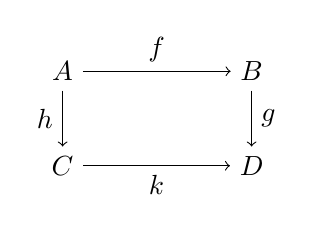
\begin{tikzpicture}[x=0.8cm, y=0.6cm]
        \node (FX) at (0, 2) {$A$};
        \node (FY) at (0, 0) {$C$};
        \node (GX) at (3, 2) {$B$};
        \node (GY) at (3, 0) {$D$};
        \draw[->] (FX) -- node[above]{$f$} (GX);
        \draw[->] (FX) -- node[left] {$h$} (FY);
        \draw[->] (FY) -- node[below]{$k$} (GY);
        \draw[->] (GX) -- node[right]{$g$} (GY);
    \end{tikzpicture}
    \end{center}
    is said to be \textbf{commute} if $g\circ f=k\circ h$.
\end{definition}

\begin{definition}
    Let $\mathcal{C}$ and $\mathcal{D}$ be categories with $\ob\mathcal{D}\subseteq\ob\mathcal{C}$.
    \begin{enumerate}
        \item $\mathcal{D}$ is a \textbf{subcategory} of $\mathcal{C}$ if for all $X, Y\in\ob\mathcal{D}$,
        \[
            \hom_{\mathcal{D}}(X, Y)\subseteq\hom_\mathcal{C}(X, Y).
        \]
        \item $\mathcal{D}$ is a \textbf{full subcategory} of $\mathcal{C}$ if for all $X, Y\in\ob\mathcal{D}$,
        \[
            \hom_{\mathcal{D}}(X, Y)=\hom_\mathcal{C}(X, Y).
        \]
    \end{enumerate}
\end{definition}

\begin{definition}
    The \textbf{product category} $\mathcal{C}\times\mathcal{D}$ of $\mathcal{C}$ and $\mathcal{D}$ is defined by:
    \begin{enumerate}
        \item $\ob(\mathcal{C}\times\mathcal{D})=\{(X, Y)\ |\ X\in\ob\mathcal{C}\text{ and }Y\in\ob\mathcal{D}\}$.
        \item $\hom((X, Y), (X', Y'))=\{(f, g)\ |\ f:X\to X'\text{ and }g:Y\to Y'\}$.
        \item $(f, g)\circ(h, k)=(f\circ h, g\circ k)$.
    \end{enumerate}
\end{definition}

\subsection{Functors}

Let $\mathcal{C}$ and $\mathcal{D}$ be categories.

\begin{definition}
    A \textbf{functor} $F:\mathcal{C}\to\mathcal{D}$ consists of:
    \begin{enumerate}
        \item A function $F:\ob\mathcal{C}\to\ob\mathcal{D}$.
        \item For $X, Y\in\ob\mathcal{C}$, a function $F_{X, Y}:\hom_\mathcal{C}(X, Y)\to\hom_\mathcal{D}(F(X), F(Y))$.
        \item $F_{X, X}(1_X)=1_{F(X)}$ for $X\in\ob\mathcal{C}$.
        \item $F_{X, Z}(g\circ_\mathcal{C} f)=F_{Y, Z}(g)\circ_\mathcal{D}F_{X, Y}(f)$ for $f:X\to Y$ and $g:Y\to Z$.
    \end{enumerate}
\end{definition}

In other words, the diagram commute:
\begin{center}
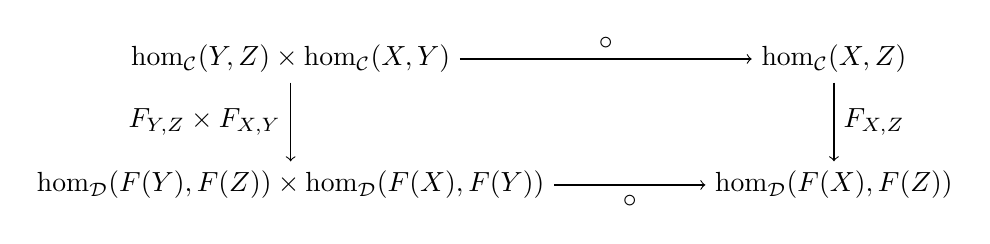
\begin{tikzpicture}[x=2.3cm, y=0.8cm]
    \node (FX) at (0, 2) {$\hom_\mathcal{C}(Y, Z)\times\hom_\mathcal{C}(X, Y)$};
    \node (FY) at (0, 0) {$\hom_\mathcal{D}(F(Y), F(Z))\times\hom_\mathcal{D}(F(X), F(Y))$};
    \node (GX) at (3, 2) {$\hom_\mathcal{C}(X, Z)$};
    \node (GY) at (3, 0) {$\hom_\mathcal{D}(F(X), F(Z))$};
    \draw[->] (FX) -- node[above]{$\circ$} (GX);
    \draw[->] (FX) -- node[left] {$F_{Y, Z}\times F_{X, Y}$} (FY);
    \draw[->] (FY) -- node[below]{$\circ$} (GY);
    \draw[->] (GX) -- node[right]{$F_{X, Z}$} (GY);
\end{tikzpicture}
\end{center}

The functor will be expressed as
\[
    F:\mathcal{C}\to\mathcal{D}:X\mapsto FX:f\mapsto Ff
\]
Parentheses are omitted unless symbolic clarity is required.

\begin{definition}
    Let $F:\mathcal{C}\to\mathcal{D}$ and $G:\mathcal{D}\to\mathcal{E}$ be functors.
    The \textbf{composite} of $F$ and $G$ are defined by
    \[
        GF = G\circ F:\mathcal{C}\to\mathcal{E}:X\mapsto GFX:f\mapsto GFf.
    \]
\end{definition}

\begin{definition}
    The \textbf{category of categories} \textbf{Cat} is defined by:
    \begin{enumerate}
        \item $\ob\textbf{Cat} = \{\mathcal{C}\ |\ \mathcal{C}\text{ is a category}\}$.
        \item $\hom(\mathcal{C}, \mathcal{D})=\{F:\mathcal{C}\to\mathcal{D}\ |\ F\text{ is a functor}\}$.
    \end{enumerate}
\end{definition}

Then the product defines a functor $\times:\textbf{Cat}\times\textbf{Cat}\to\textbf{Cat}$.

\begin{definition}
    Let $F:\mathcal{C}\to\mathcal{D}$ be a functor.
    \begin{enumerate}
        \item $F$ is \textbf{faithful} if all $F_{X, Y}$ are injective.
        \item $F$ is \textbf{full} if all $F_{X, Y}$ are surjective.
        \item $F$ is \textbf{fully faithful} if all $F_{X, Y}$ are bijective.
    \end{enumerate}
\end{definition}

A faithful functor may map two objects to the same object.

\begin{property}
    The following are equivalent for a functor $F:\mathcal{C}\to\mathcal{D}$:
    \begin{enumerate}
        \item $F$ is fully faithful and bijective on objects.
        \item There is a functor $G:\mathcal{D}\to\mathcal{C}$ such that $G\circ F=1_\mathcal{C}$ and $F\circ G=1_\mathcal{D}$.
    \end{enumerate}
    In this case, $F$ is called an \textbf{isomorphism} between categories.
\end{property}

\subsection{Naturality}

\begin{definition}
    Let $F, G:\mathcal{C}\to\mathcal{D}$ be functors.
    A \textbf{(natural) transformation} $\alpha:F\Rightarrow G$ is a function $$\alpha:\ob(\mathcal{C})\to\hom(\mathcal{D}):X\mapsto\alpha_X$$ such that the following diagram commutes:
    \begin{center}
    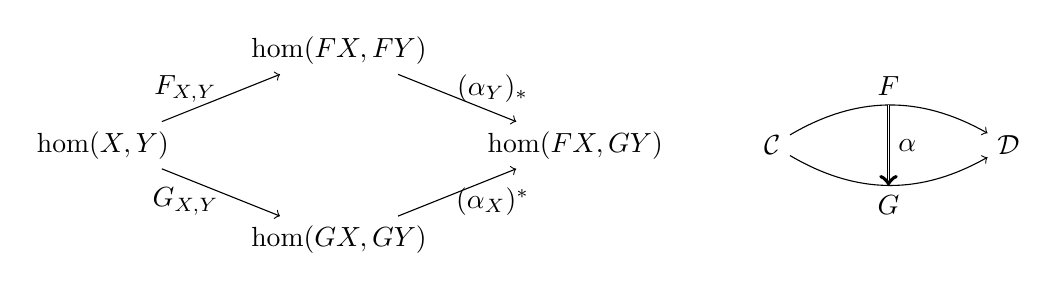
\begin{tikzpicture}[x=1cm, y=0.6cm]
        \node (FX) at (0, 0) {$\hom(X, Y)$};
        \node (FY) at (3,-2) {$\hom(GX, GY)$};
        \node (GX) at (3, 2) {$\hom(FX, FY)$};
        \node (GY) at (6, 0) {$\hom(FX, GY)$};
        \draw[->] (FX) -- node[above, pos=0.2]{$F_{X, Y}$} (GX);
        \draw[->] (FX) -- node[below, pos=0.2] {$G_{X, Y}$} (FY);
        \draw[->] (FY) -- node[below, pos=0.8]{$(\alpha_X)^*$} (GY);
        \draw[->] (GX) -- node[above, pos=0.8]{$(\alpha_Y)_*$} (GY);
        
        \node (C)  at ( 8.5, 0) {$\mathcal{C}$};
        \node (D)  at (11.5, 0) {$\mathcal{D}$};
        \draw[->,bend  left] (C) edge node[above]{$F$} coordinate(F) (D);
        \draw[->,bend right] (C) edge node[below]{$G$} coordinate(G) (D);
        \draw[->,double] (F) -- node[right]{$\alpha$} (G);
    \end{tikzpicture}
    \end{center}
    In other words, $\alpha_Y\circ Ff=Gf\circ\alpha_X$ for each $f:X\to Y$.
    \begin{center}
    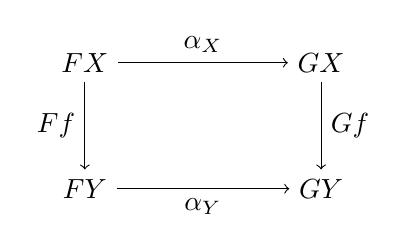
\begin{tikzpicture}[x=1cm, y=0.8cm]
        \node (FX) at (0, 2) {$FX$};
        \node (FY) at (0, 0) {$FY$};
        \node (GX) at (3, 2) {$GX$};
        \node (GY) at (3, 0) {$GY$};
        \draw[->] (FX) -- node[above]{$\alpha_X$} (GX);
        \draw[->] (FX) -- node[left] {$Ff$} (FY);
        \draw[->] (FY) -- node[below]{$\alpha_Y$} (GY);
        \draw[->] (GX) -- node[right]{$Gf$} (GY);
    \end{tikzpicture}
    \end{center}
\end{definition}

\begin{definition}
    The \textbf{vertical composition} $\beta\circ\alpha:F\Rightarrow H$ of transformations $\alpha:F\Rightarrow G$ and $\beta:G\Rightarrow H$ is defined by 
        \begin{center}
        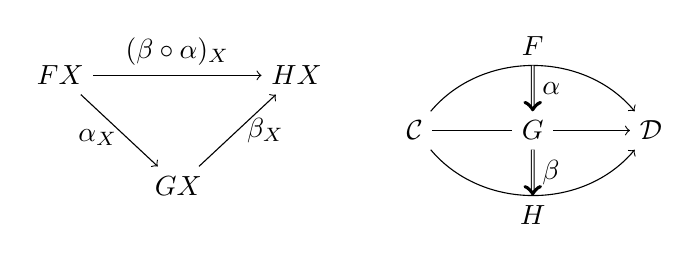
\begin{tikzpicture}[x=1.5cm, y=0.7cm]
            \node (FX) at (0, 2) {$FX$};
            \node (HX) at (2, 2) {$HX$};
            \node (GX) at (1, 0) {$GX$};
            \node (C)  at (3, 1) {$\mathcal{C}$};
            \node (D)  at (5, 1) {$\mathcal{D}$};
            \node (G)  at (4, 1) {$G$};
            \draw[->] (FX) -- node[ left, pos=0.6] {$\alpha_X$} (GX);
            \draw[->] (FX) -- node[above] {$(\beta\circ\alpha)_X$} (HX);
            \draw[->] (GX) -- node[right] {$\beta_X$} (HX);
            \draw[->,bend left=50] (C) edge node[above] {$F$} coordinate(F) (D);
            \draw (C) -- (G);
            \draw[->]  (G) -- (D);
            \draw[->,bend right=50] (C) edge node[below] {$H$} coordinate(H) (D);
            \draw[->, double] (F) -- node[right] {$\alpha$} (G);
            \draw[->, double] (G) -- node[right] {$\beta$} (H);
        \end{tikzpicture}
        \end{center}
\end{definition}

\begin{definition}
    The \textbf{functor category} $[\mathcal{C}, \mathcal{D}]$ is defined by:
    \begin{enumerate}
        \item $\ob[\mathcal{C}, \mathcal{D}]=\{F:\mathcal{C}\to\mathcal{D}\ |\ F\text{ is a functor}\}$.
        \item $\hom(F, G)=\{\alpha:F\Rightarrow G\ |\ \alpha\text{ is a natural transformation}\}$.
        \item The composition in functor category is defined vertically.
    \end{enumerate}
    Then we have a functor $[-, -]:\textbf{Cat}^{op}\times\textbf{Cat}\to\textbf{Cat}$.
\end{definition}

\begin{definition}
    The \textbf{horizontal composition} is a functor
    \[
        *:
        [\mathcal{D}, \mathcal{E}]\times[\mathcal{C}, \mathcal{D}] \to [\mathcal{C}, \mathcal{E}]:
        (J, F) \mapsto JF:
        (\beta, \alpha) \mapsto \beta*\alpha
    \]
    where $\beta*\alpha:JF\to KG$ is defined by
        
        \begin{center}
        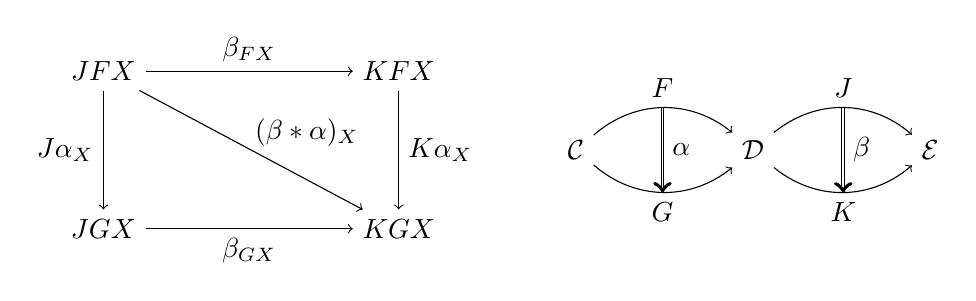
\begin{tikzpicture}[x=1.5cm, y=2cm]
            \node (HFX) at (0.5, 1) {$JFX$};
            \node (KFX) at (3, 1) {$KFX$};
            \node (HGX) at (0.5, 0) {$JGX$};
            \node (KGX) at (3, 0) {$KGX$};
            \draw[->] (HFX) -- node[right, pos=0.35] {$\hspace{10pt}(\beta*\alpha)_X$} (KGX);
            \draw[->] (HFX) -- node[above] {$\beta_{FX}$} (KFX);
            \draw[->] (HFX) -- node[ left] {$J\alpha_X$}  (HGX);
            \draw[->] (KFX) -- node[right] {$K\alpha_X$}  (KGX);
            \draw[->] (HGX) -- node[below] {$\beta_{GX}$} (KGX);
            
            \node (C)  at (4.5, 0.5) {$\mathcal{C}$};
            \node (D)  at (6, 0.5) {$\mathcal{D}$};
            \node (E)  at (7.5, 0.5) {$\mathcal{E}$};
            \draw[->,bend  left=40] (C) edge node[above]{$F$} coordinate(F) (D);
            \draw[->,bend right=40] (C) edge node[below]{$G$} coordinate(G) (D);
            \draw[->,double] (F) -- node[right]{$\alpha$} (G);
            \draw[->,bend  left=40] (D) edge node[above]{$J$} coordinate(J) (E);
            \draw[->,bend right=40] (D) edge node[below]{$K$} coordinate(K) (E);
            \draw[->,double] (J) -- node[right]{$\beta$} (K);
        \end{tikzpicture}
        \end{center}
\end{definition}

\begin{property}
    Let $\alpha, \beta, \delta, \gamma$ be natural transformations.
    \begin{enumerate}
        \item $\beta*\alpha=(1_K*\alpha)\circ(\beta*1_F)=(\beta*1_G)\circ(1_J*\alpha)$.
        \item $(\delta\circ\beta)*(\gamma\circ\alpha)=(\delta*\gamma)\circ(\beta*\alpha)$.
        \item $\gamma*(\beta*\alpha)=(\gamma*\beta)*\alpha$. 
    \end{enumerate} 
    \begin{center}
    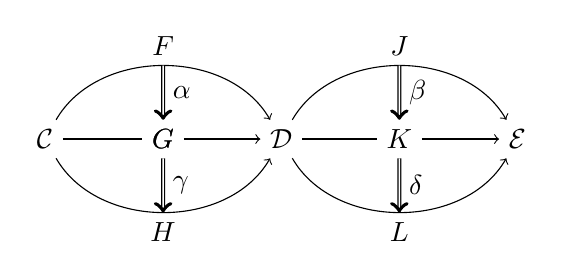
\begin{tikzpicture}[x=1.5cm, y=1cm]
        % \node (JF) at (0, 1) {$JF$};
        % \node (KF) at (2, 1) {$KF$};
        % \node (JG) at (0,-1) {$JG$};
        % \node (KG) at (2,-1) {$KG$};
        % \draw[->] (JF) -- node[right, pos=0.35] {$\hspace{10pt}\beta*\alpha$} (KG);
        % \draw[->] (JF) -- node[above] {$\beta*1_F$} (KF);
        % \draw[->] (JF) -- node[ left] {$1_J*\alpha$}  (JG);
        % \draw[->] (KF) -- node[right] {$1_K*\alpha$}  (KG);
        % \draw[->] (JG) -- node[below] {$\beta*1_G$} (KG);

        \node (C)  at (3, 1) {$\mathcal{C}$};
        \node (D)  at (5, 1) {$\mathcal{D}$};
        \node (G)  at (4, 1) {$G$};
        \draw[->,bend left=60] (C) edge node[above](F) {$F$} (D);
        \draw (C) -- (G);
        \draw[->] (G) -- (D);
        \draw[->,bend right=60] (C) edge node[below](H) {$H$} (D);
        \draw[->, double] (F) -- node[right]{$\alpha$} (G);
        \draw[->, double] (G) -- node[right]{$\gamma$} (H);
        \node (E)  at (7, 1) {$\mathcal{E}$};
        \node (G)  at (4, 1) {$G$};
        \node (K)  at (6, 1) {$K$};
        \draw[->,bend left=60] (D) edge node[above](J) {$J$} (E);
        \draw (D) -- (K);
        \draw[->] (K) -- (E);
        \draw[->,bend right=60] (D) edge node[below](L) {$L$} (E);
        \draw[->, double] (J) -- node[right]{$\beta$} (K);
        \draw[->, double] (K) -- node[right]{$\delta$} (L);
    \end{tikzpicture}
    \end{center}
\end{property}

\subsection{Monics and Epis}

\begin{definition}
    Let $f:X\to Y$ and $Z\in\ob\mathcal{C}$.
    The \textbf{post-composition} of $f$ is defined by $$f_*:\hom(Z, X)\to\hom(Z, Y):g\mapsto f\circ g,$$ and the \textbf{pre-composition} of $f$ is defined by $$f^*:\hom(Y, Z)\to\hom(X, Z):h\mapsto h\circ f.$$
    \begin{center}
    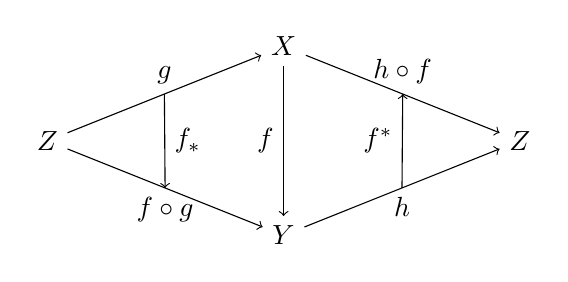
\begin{tikzpicture}[x=1cm, y=0.6cm]
        \node (X)  at ( 0, 4) {$X$};
        \node (Y)  at ( 0, 0) {$Y$};
        \node (Zr) at ( 3, 2) {$Z$};
        \node (Zl) at (-3, 2) {$Z$};
        \draw[->]   (X) -- node [left]{$f$} (Y);
        \draw[->]   (X) -- node[above]{$h\circ f$} coordinate(XZr) (Zr);
        \draw[->]   (Y) -- node[below]{$h$} coordinate(YZr) (Zr);
        \draw[->]  (Zl) -- node[above]{$g$} coordinate(XZl) (X);
        \draw[->]  (Zl) -- node[below]{$f\circ g$} coordinate(YZl) (Y);
        \draw[->] (YZr) -- node [left]{$f^*$} (XZr);
        \draw[->] (XZl) -- node[right]{$f_*$} (YZl);
    \end{tikzpicture}
    \end{center}
\end{definition}
\begin{center}
\begin{tabular}{l|l}
    Types of Morphisms & Conditions for $f:X\to Y$ \\
    \hline \\[-12pt]
    monomorphism / monic & $f_*$ is injective \\
    epimorphism  / epic  & $f^*$ is injective \\
    bimorphism   & $f$ is monic and epic \\
    split monomorphism   & $f^*$ is surjective \\
    split epimorphism    & $f_*$ is surjective \\
    isomorphism  & $f^*$ or $f_*$ is bijective \\
    endomorphism & $X=Y$ \\
    automorphism & $f$ is an isomorphism and $X=Y$
\end{tabular}
\end{center}

We write $f:X\rightarrowtail Y$ for monomorphisms and $f:X\twoheadrightarrow Y$ for epimorphisms.

Examples:
\begin{center}
    \begin{tabular}{c|c}
        Types of Morphisms & Morphisms in \textbf{Set} \\
        \hline
        monomorphism & injection \\
        epimorphism  & surjection \\
        split monomorphism & injection with a non-empty domain \\
        split epimorphism & surjection \\
        isomorphism   & bijection \\
        automorphism  & permutation
    \end{tabular}
\end{center}

\begin{property}
    Let $f:X\to Y$ and $g:Y\to Z$ be morphisms.
    \begin{enumerate}
        \item If $f, g$ are monic(epic), then $g\circ f$ is monic(epic).
        \item If $g\circ f$ is monic, then $f$ is monic.
        \item If $g\circ f$ is epic, then $g$ is epic.
        \item Split monomorphisms are monic, split epimorphisms are epic.
        \item $f$ is a split monomorphism $\iff f$ has a left inverse.
        \item $f$ is a split epimorphism $\iff f$ has a right inverse.
        \item $f$ is an isomorphism $\iff f$ has a two-sided inverse.
    \end{enumerate}
\end{property}

\begin{lemma}
\label{FF functor}
    Let $\mathcal{C}$ be a category.
    \begin{enumerate}
        \item Functors preserve split monomorphisms and split epimorphisms.
        \item Faithful functors reflect monics and epics.
        \item Full and faithful functors reflect split monics and split epics.
    \end{enumerate}
\end{lemma}

\begin{definition}
    A \textbf{natural isomorphism} $\alpha:F\cong G$ is a transformation $\alpha:F\Rightarrow G$ that satisfies the following equivalent consitions:
    \begin{enumerate}
        \item $\alpha$ is an isomorphism in the functor category.
        \item Every component of $\alpha$ is an isomorphism.
    \end{enumerate}
\end{definition}

\subsection{Duality}

\begin{definition}
    The \textbf{opposite category} $\mathcal{C}^{op}$ of $\mathcal{C}$ is defined by:
    \begin{enumerate}
        \item $\ob\mathcal{C}^{op}=\ob\mathcal{C}$.
        \item $\hom_{\mathcal{C}^{op}}(X, Y)=\hom_\mathcal{C}(Y, X)$ for all $X$ and $Y$.
        \item The composition $$\circ:\hom_{\mathcal{C}^{op}}(Y, Z)\times\hom_{\mathcal{C}^{op}}(X, Y)\to\hom_{\mathcal{C}^{op}}(X, Z)$$ is given by $\circ:\hom_\mathcal{C}(Y, X)\times\hom_\mathcal{C}(Z, Y)\to\hom_\mathcal{C}(Z, X)$.
    \end{enumerate}
\end{definition}

Note that the assignment
\[
    (-)^{op}:\mathcal{C}\to\mathcal{C}^{op}:(f:X\to Y)\mapsto(f:Y\to X)
\]
is \textbf{not} a functor; it satisfies $f^{op}\circ g^{op}=(g\circ f)^{op}$.

\begin{definition}
    Let $F:\mathcal{C}\to\mathcal{D}$ be a functor.
    \begin{enumerate}
        \item $F$ is called a \textbf{covariant functor} from $\mathcal{C}$ to $\mathcal{D}$.
        \item $F$ is called a \textbf{contravariant functor} from $\mathcal{C}^{op}$ to $\mathcal{D}$.
        \item The \textbf{opposite functor} of $F$ is
        \[
            F^{op}:\mathcal{C}^{op}\to\mathcal{D}^{op}:X\mapsto FX:f^{op}\mapsto(Ff)^{op}.
        \]
    \end{enumerate}
\end{definition}

\begin{property}
    Let $f:X\to Y$ be a morphism in $\mathcal{C}$.
    \begin{enumerate}
        \item $f$ is monic $\iff f^{op}$ is epic.
        \item $f$ is split monic $\iff f^{op}$ is split epic.
    \end{enumerate}
\end{property}

\subsection{Terminology and Constructions}

\begin{definition}
    Let $\mathcal{C}$ be a category.
    \begin{enumerate}
        \item $\mathcal{C}$ is a \textbf{groupoid} if all its morphisms are isomorphisms.
        \item $\mathcal{C}$ is \textbf{discrete} if all its morphisms are identities.
        \item $\mathcal{C}$ is \textbf{skeletal} if all its isomorphisms are automorphisms.
        \item $\mathcal{C}$ is \textbf{thin} if all its hom-sets contains at most one morphism.
        \item $\mathcal{C}$ is \textbf{connected} if all functor from $\mathcal{C}$ to a discrete category is constant.
        \item $\mathcal{C}$ is \textbf{concrete} if there is a faithful functor from $\mathcal{C}$ to \textbf{Set}
    \end{enumerate}
\end{definition}

\begin{corollary}
    A thin category is the same thing as a preordered set, a thin skeletal category is the same thing as a partially ordered set, and a thin, connected skeletal category is the same thing as a linearly ordered set.
\end{corollary}

\begin{definition}
    Let $\mathcal{J}$ and $\mathcal{C}$ be categories.
    Define 
    \[
        \Delta X:\mathcal{J}\to\mathcal{C}:A\mapsto X:g\mapsto 1_X
        \quad\text{and}\quad
        \Delta f:\Delta X\Rightarrow\Delta Y:A\mapsto f
    \]
    for all $f:X\to Y$ in $\mathcal{C}$.
    Then
    \[
        \Delta:
        \mathcal{C}\to[\mathcal{J}, \mathcal{C}]:
        X\mapsto \Delta X:
        f\mapsto \Delta f
    \]
    is called the \textbf{diagonal functor} or \textbf{constant functor}.
\end{definition}

Note that $\Delta$ is fully faithful.

\begin{definition}
    Let $F:\mathcal{C}_1\to\mathcal{D}$ and $G:\mathcal{C}_2\to\mathcal{D}$ be functors.
    The \textbf{comma category} $F\downarrow G$ is defined by:
    \begin{enumerate}
        \item $\ob(F\downarrow G)=\{f:FX\to GY\ |\ (X, Y)\in\ob(\mathcal{C}_1\times\mathcal{C}_2)\}$.
        \item $\hom(f, g)=\{(h, k)\ |\ g\circ Fh=Gk\circ f\}$.
    \end{enumerate}
    \begin{center}
    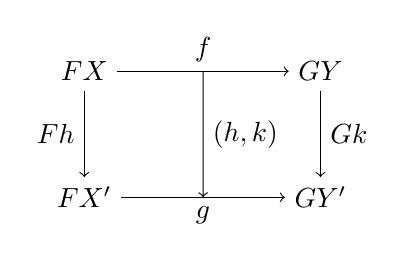
\begin{tikzpicture}[x=1cm, y=0.8cm]
        \node (Fd)  at (0, 2) {$FX$};
        \node (Fd') at (0, 0) {$FX'$};
        \node (Ge)  at (3, 2) {$GY$};
        \node (Ge') at (3, 0) {$GY'$};
        \draw[->] (Fd)  -- node[above]{$f$}     coordinate(f)  (Ge);
        \draw[->] (Fd)  -- node[left] {$Fh$} (Fd');
        \draw[->] (Fd') -- node[below]{$g$}    coordinate(f') (Ge');
        \draw[->] (Ge)  -- node[right]{$Gk$} (Ge');
        \draw[->] (f)  -- node[right]{$(h, k)$} (f');
    \end{tikzpicture}
    \end{center}
\end{definition}

If $F\cong F'$ and $G\cong G'$, then $F\downarrow G\cong F'\downarrow G'$.

\begin{definition}
    Let $F:\mathcal{C}\to\textbf{Set}$ be a functor.
    The \textbf{category of elements} $\int F$ of $F$ is defined by:
    \begin{enumerate}
        \item $\ob\int F=\{(X, a)\ |\ X\in\ob\mathcal{C}\text{ and }a\in FX\}$.
        \item $\hom((X, a), (Y, b))=\{f:X\to Y\ |\ Ff(a)=b\}$.
    \end{enumerate}
\end{definition}

\section{Yoneda Lemma}

\subsection{Hom Functors}

\begin{definition}
    The following functors are called \textbf{hom functors}:
    \[
        \hom_\mathcal{C}(Z, -): \mathcal{C}\to\textbf{Set}: X\mapsto\hom_\mathcal{C}(Z, X): f\mapsto f_*
    \]
    \[
        \hom_\mathcal{C}(-, Z): \mathcal{C}^{op}\to\textbf{Set}: X\mapsto\hom_\mathcal{C}(X, Z): f\mapsto f^*
    \]
    \[
        \hom_\mathcal{C}(-, -): \mathcal{C}^{op}\times\mathcal{C}\to\textbf{Set}: (X, Y)\to\hom_\mathcal{C}(W, Z): (f, h)\mapsto f^*\circ h_*
    \]
    \begin{center}
    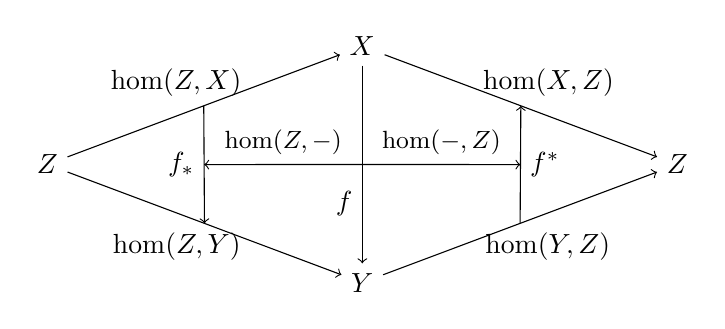
\begin{tikzpicture}[x=1cm, y=0.6cm]
        \node (X)  at ( 0, 5) {$X$};
        \node (Y)  at ( 0, 0) {$Y$};
        \node (Zr) at ( 4, 2.5) {$Z$};
        \node (Zl) at (-4, 2.5) {$Z$};
        \draw[->] (X)   -- node[left, pos=0.7]{$f$} coordinate(XY) (Y);
        \draw[->] (X)   -- node[above]{$\qquad\hom(X, Z)$} coordinate(XZr) (Zr);
        \draw[->] (Y)   -- node[below]{$\qquad\hom(Y, Z)$} coordinate(YZr) (Zr);
        \draw[->] (Zl)  -- node[above]{$\hom(Z, X)\qquad$} coordinate(XZl) (X);
        \draw[->] (Zl)  -- node[below]{$\hom(Z, Y)\qquad$} coordinate(YZl) (Y);
        \draw[->] (YZr) -- node[right]{$f^*$} coordinate(HOMr) (XZr);
        \draw[->] (XZl) -- node[left] {$f_*$} coordinate(HOMl) (YZl);
        \draw[->] (XY)  -- node[above]{\small$\hom(-, Z)$} (HOMr);
        \draw[->] (XY)  -- node[above]{\small$\hom(Z, -)$} (HOMl);
    \end{tikzpicture}
    \end{center}
\end{definition}

\begin{property}
    Let $F:\mathcal{C}\to\mathcal{D}$ be a functor.
    Define
    \[
        \hom_F:\hom_\mathcal{C}(-, -)\Rightarrow\hom_\mathcal{D}(F^{op}-, F-):
        (X, Y)\mapsto F_{X, Y}.
    \]
    \begin{enumerate}
        \item $F$ is faithful $\iff$ each component of $\hom_F$ is monic.
        \item $F$ is full $\iff$ each component of $\hom_F$ is epic.
        \item $F$ is fully faithful $\iff\hom_F:\hom_\mathcal{C}(-, -)\cong\hom_\mathcal{D}(F^{op}-, F-)$.
    \end{enumerate}
\end{property}

\begin{property}
    Every morphism $f:X\to Y$ defines two transformations:
    \[
        f_*:\hom(-, X)\Rightarrow\hom(-, Y)
        \quad\text{and}\quad
        f^*:\hom(Y, -)\Rightarrow\hom(X, -).
    \]
    \begin{center}
    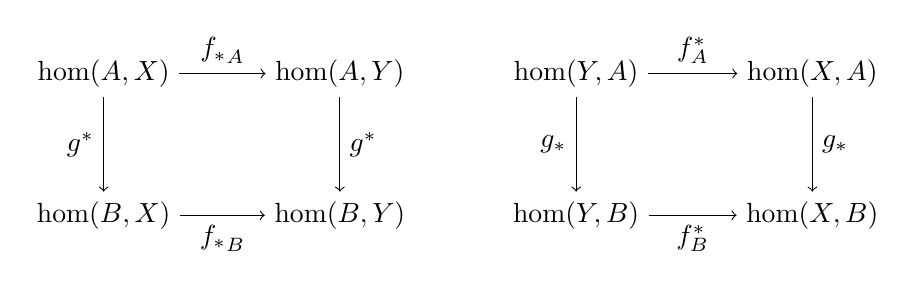
\begin{tikzpicture}[x=1cm, y=0.6cm]
        \node (AX)  at ( 0, 3) {$\hom(A, X)$};
        \node (BX)  at ( 0, 0) {$\hom(B, X)$};
        \node (AY)  at ( 3, 3) {$\hom(A, Y)$};
        \node (BY)  at ( 3, 0) {$\hom(B, Y)$};
        \draw[->] (AX) -- node[left] {$g^*$} (BX);
        \draw[->] (AY) -- node[right]{$g^*$} (BY);
        \draw[->] (AX) -- node[above]{${f_*}_A$} (AY);
        \draw[->] (BX) -- node[below]{${f_*}_B$} (BY);
        \node (YA)  at ( 6, 3) {$\hom(Y, A)$};
        \node (YB)  at ( 6, 0) {$\hom(Y, B)$};
        \node (XA)  at ( 9, 3) {$\hom(X, A)$};
        \node (XB)  at ( 9, 0) {$\hom(X, B)$};
        \draw[->] (XA) -- node[right]{$g_*$} (XB);
        \draw[->] (YA) -- node[left] {$g_*$} (YB);
        \draw[->] (YA) -- node[above]{$f^*_A$} (XA);
        \draw[->] (YB) -- node[below]{$f^*_B$} (XB);
    \end{tikzpicture}
    \end{center}
\end{property}

\begin{definition}
    The two functors are called the \textbf{Yoneda Embeddings}:
    \[
        y: \mathcal{C}^{op}\to[\mathcal{C}, \textbf{Set}]: X\mapsto\hom_\mathcal{C}(X, -): f\mapsto f^*
    \]
    \[
        y': \mathcal{C}\to[\mathcal{C}^{op}, \textbf{Set}]: X\mapsto\hom_\mathcal{C}(-, X): f\mapsto f_*
    \]
\end{definition}

\subsection{The Yoneda Lemma}

We do not distinguish between $y^{op}$ and $y$ here.

\begin{lemma}[Yoneda]
    Let $\mathcal{C}$ be a category, then
    \[
        \hom_{[\mathcal{C}, \textbf{Set}]}(yX, F) 
        \cong FX
    \]
    for all $X\in\ob\mathcal{C}$ and $F:\mathcal{C}\to\textbf{Set}$.
\end{lemma}
\begin{proof}
    Let $\alpha:\hom_\mathcal{C}(X, -)\Rightarrow F$, then the following diagram commute:
    \begin{center}
    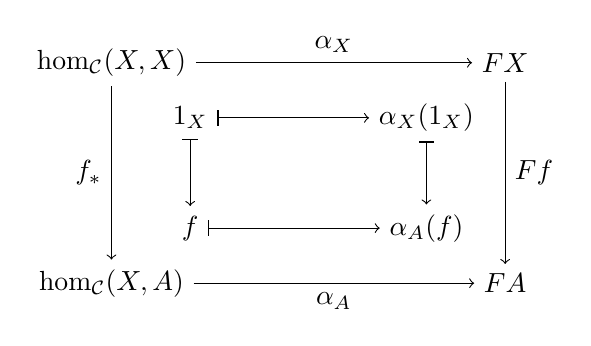
\begin{tikzpicture}[x=1cm, y=0.7cm]
        \node (1x)  at (1, 3) {$1_X$};
        \node (f)   at (1, 1) {$f$};
        \node (a1)  at (4, 3) {$\alpha_X(1_X)$};
        \node (aAf) at (4, 1) {$\alpha_A(f)$};
        \node (hxX) at (0, 4) {$\hom_\mathcal{C}(X, X)$};
        \node (hxY) at (0, 0) {$\hom_\mathcal{C}(X, A)$};
        \node (FX)  at (5, 4) {$FX$};
        \node (FY)  at (5, 0) {$FA$};
        \draw[->] (hxX) -- node[left]  {$f_*$} (hxY);
        \draw[->] (FX)  -- node[right] {$Ff$}       (FY);
        \draw[->] (hxX) -- node[above] {$\alpha_X$}  (FX);
        \draw[->] (hxY) -- node[below] {$\alpha_A$}  (FY);
        \draw[|->] (1x) --  (a1);
        \draw[|->] (1x) --  (f);
        \draw[|->] (a1) --  (aAf);
        \draw[|->] (f)  --  (aAf);
    \end{tikzpicture}
    \end{center}
    It follows that $\alpha_A(f)=Ff(\alpha_X(1_X))$ and all the component $\alpha_A$ of $\alpha$ must defined by
    \[
        \alpha_A:\hom_\mathcal{C}(X, A)\to FA: f\mapsto Ff(\alpha_X(1_X)).
    \]
    Therefore, the natural transformation $\alpha:yX\Rightarrow F$ is completely determined by $\alpha_X(1_X)\in FX$.
    Note that the inverse of
    \[
        \Phi:\hom_{[\mathcal{C}, \textbf{Set}]}(yX, F) \to FX:
        \Big(\alpha:yX\Rightarrow F\Big) \mapsto \alpha_X(1_X)
    \]
    is defined by $\Psi:FX\to\hom_{[\mathcal{C}, \textbf{Set}]}(yX, F)$ with
    \[
        \Psi(a)_A:\hom_\mathcal{C}(X, A)\to FA:\Big(f:X\to A\Big)\mapsto Ff(a).
    \]
\end{proof}

The dual version of Yoneda Lemma
\[
    \hom_{[\mathcal{C}, \textbf{Set}]}(y'X, F)\cong FX
\]
is proved by the following diagram:
\begin{center}
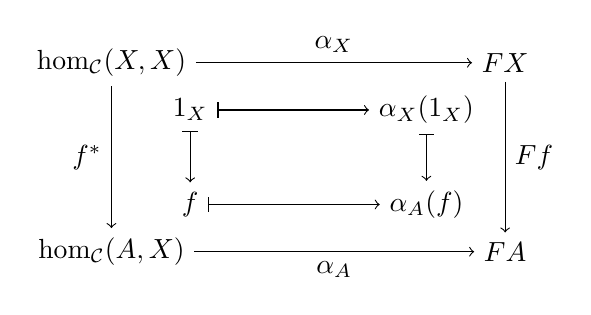
\begin{tikzpicture}[x=1cm, y=0.6cm]
    \node (1x)  at (1, 3) {$1_X$};
    \node (f)   at (1, 1) {$f$};
    \node (a1)  at (4, 3) {$\alpha_X(1_X)$};
    \node (aAf) at (4, 1) {$\alpha_A(f)$};
    \node (hxX) at (0, 4) {$\hom_\mathcal{C}(X, X)$};
    \node (hxY) at (0, 0) {$\hom_\mathcal{C}(A, X)$};
    \node (FX)  at (5, 4) {$FX$};
    \node (FY)  at (5, 0) {$FA$};
    \draw[->] (hxX) -- node[left]  {$f^*$} (hxY);
    \draw[->] (FX)  -- node[right] {$Ff$}       (FY);
    \draw[->] (hxX) -- node[above] {$\alpha_X$}  (FX);
    \draw[->] (hxY) -- node[below] {$\alpha_A$}  (FY);
    \draw[|->] (1x) --  (a1);
    \draw[|->] (1x) --  (f);
    \draw[|->] (a1) --  (aAf);
    \draw[|->] (f)  --  (aAf);
\end{tikzpicture}
\end{center}

\begin{property}
    Define the \textbf{evaluation functor}
    \[
        Ev:
        \mathcal{C}\times[\mathcal{C}, \textbf{Set}]\to\textbf{Set}:
        (X, F)\mapsto FX:
        (f, \gamma)\mapsto Gf\circ\gamma_X=\gamma_Y\circ Ff.
    \]
    Then
    \[
        \Phi:\hom_{[\mathcal{C}, \textbf{Set}]}(y-, -)\cong Ev(-, -):\Psi.
    \]
\end{property}
\begin{proof}
    % To prove that the diagram commute
    Let $f:X\to Y$ in $\mathcal{C}$ and $\gamma:F\Rightarrow G$.
    For each $\alpha:\hom_\mathcal{C}(X, -)\Rightarrow F$, we have $\alpha_Y(f)=Ff(\alpha_X(1_X))$.
    Then the following diagram commute:
    \begin{center}
    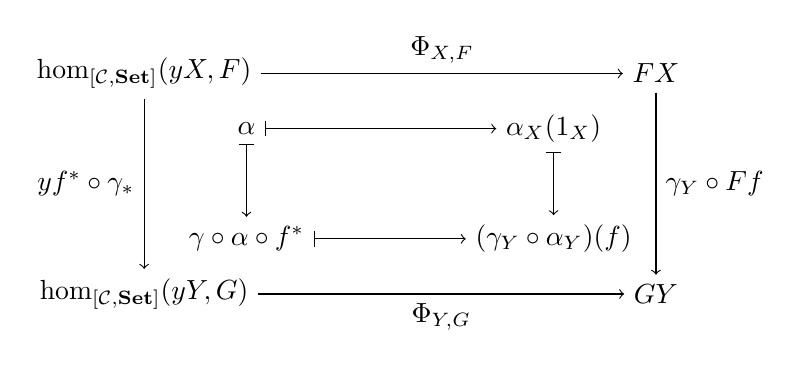
\begin{tikzpicture}[x=1.3cm, y=0.7cm]
        \node (hxF) at (0, 4) {$\hom_{[\mathcal{C}, \textbf{Set}]}(yX, F)$};
        \node (hxG) at (0, 0) {$\hom_{[\mathcal{C}, \textbf{Set}]}(yY, G)$};
        \node (FX)  at (5, 4) {$FX$};
        \node (GX)  at (5, 0) {$GY$};
        \node (a) at (1, 3) {$\alpha$};
        \node (ax) at (4, 3) {$\alpha_X(1_X)$};
        \node (gaf) at (1, 1) {$\gamma\circ\alpha\circ f^*$};
        \node (ga) at (4, 1) {$(\gamma_Y\circ\alpha_Y)(f)$};
        \draw[->] (hxF) -- node[left]  {$yf^*\circ\gamma_*$} (hxG);
        \draw[->] (FX)  -- node[right] {$\gamma_Y\circ Ff$} (GX);
        \draw[->] (hxF) -- node[above] {$\Phi_{X, F}$}  (FX);
        \draw[->] (hxG) -- node[below] {$\Phi_{Y, G}$}  (GX);
        \draw[|->] (a) -- (ax);
        \draw[|->] (a) -- (gaf);
        \draw[|->] (ax) -- (ga);
        \draw[|->] (gaf) -- (ga);
    \end{tikzpicture}
    \end{center}
    % \begin{align*}
    %     (\gamma_Y\circ Ff\circ\Phi_{X, F})(\alpha) &
    %       = (\gamma_Y\circ Ff\circ\alpha_X)(1_X) 
    %       = (\gamma_Y\circ\alpha_Y)(f) \\
    %     & = (\gamma\circ\alpha\circ f^*)_Y(1_Y)
    %       = (\Phi_{Y, G}\circ(f^*)^*\circ\gamma_*)(\alpha).
    % \end{align*}
\end{proof}

\begin{theorem}
    The Yoneda embeddings are fully faithful.
\end{theorem}
\begin{proof}
    Apply the Yoneda lemma to the functor $yY=\hom_\mathcal{C}(Y, -)$, then
    \[
        \Psi:
        \hom_\mathcal{C}(Y, X)
        \to \hom_{[\mathcal{C}, \textbf{Set}]}(yX, yY):g\mapsto g^*.
    \]
    is a bijection.
    Since $y=\Psi$ on $\hom_\mathcal{C}(Y, X)$, $y$ is fully faithful.
\end{proof}

\begin{corollary}
\label{227}
    Let $F, G:\mathcal{C}\to\mathcal{D}$ be functors, then
    \[
        F\cong G\iff\hom_\mathcal{D}(-, F-)\cong\hom_\mathcal{D}(-, G-).
    \]
\end{corollary}
\begin{proof}
    Suppose that $\Theta:\hom_\mathcal{D}(-, F-)\cong\hom_\mathcal{D}(-, G-)$.
    Since the Yoneda embedding $y':\mathcal{D}\to[\mathcal{D}^{op}, \textbf{Set}]$ is fully faithful, for all $X\in\ob\mathcal{C}$, there is a unique isomorphism $\alpha_X:FX\to GX$ induced the isomorphism 
    \[
        y'\alpha_X=(\alpha_X)_*:\hom_\mathcal{D}(-, FX)\cong\hom_\mathcal{D}(-, GX).
    \]
    By the naturality of $\Theta$, for every morphism $f:X\to Y$ in $\mathcal{C}$, the diagram
    \begin{center}
    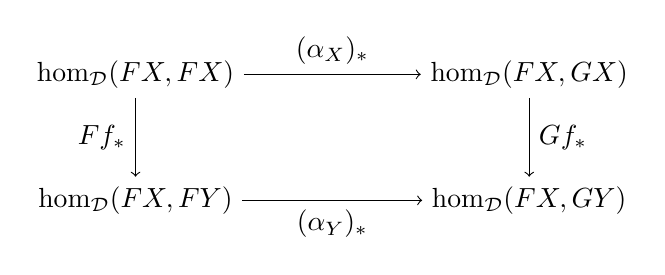
\begin{tikzpicture}[x=1cm, y=0.4cm]
        \node (hxX) at (0, 4) {$\hom_\mathcal{D}(FX, FX)$};
        \node (hxY) at (0, 0) {$\hom_\mathcal{D}(FX, FY)$};
        \node (FX)  at (5, 4) {$\hom_\mathcal{D}(FX, GX)$};
        \node (FY)  at (5, 0) {$\hom_\mathcal{D}(FX, GY)$};
        \draw[->] (hxX) -- node[left]  {$Ff_*$} (hxY);
        \draw[->] (FX)  -- node[right] {$Gf_*$} (FY);
        \draw[->] (hxX) -- node[above] {$(\alpha_X)_*$} (FX);
        \draw[->] (hxY) -- node[below] {$(\alpha_Y)_*$} (FY);
    \end{tikzpicture}
    \end{center}
    commute.
    Tracing $1_{FX}$ over the diagram, we conclude that $\alpha:F\cong G$.
\end{proof}

% \begin{definition}
%     Let $\mathcal{C}$ and $\mathcal{D}$ be categories.
%     Define
%     \begin{enumerate}
%         \item $\mathcal{D}^\mathcal{C}=\{F:\mathcal{C}\to\mathcal{D}\ |\ F\text{ is a (object) function}\}$.
%         \item $\hom(F, G)=\{\alpha:\mathcal{C}\to\hom(\mathcal{D})\ |\ \alpha(X):FX\to GX\text{ for }X\in\mathcal{C}\}$.
%     \end{enumerate}
% \end{definition}
% Note that there is a forgetful functor from $[\mathcal{C}, \mathcal{D}]$ to $\mathcal{D}^\mathcal{C}$.

% \begin{corollary}[Cayley]
%     Every group is isomorphic to a subgroup of a symmetric group.
% \end{corollary}
% \begin{proof}
%     Let $\textbf{G}=\{*\}$ be an one-object groupoid and $G$ be the hom-set in \textbf{G}.
%     Composing $y':\textbf{G}\to[\textbf{G}^{op}, \textbf{Set}]:f\mapsto f_*$ with the two forgetful functors $U_1:[\textbf{G}^{op}, \textbf{Set}]\to\textbf{Set}^{\textbf{G}^{op}}$ and $U_2:\textbf{Set}^{\textbf{G}^{op}}\to\textbf{Set}:F\mapsto F*:\alpha\mapsto\alpha(*)$, then
%     \[
%         (U_2U_1y')(*) 
%         = (U_2U_1)(\hom(-, *))
%         = \hom(*, *)
%         = G.
%     \]
%     Since functors preserve isomorphisms, $(U_2U_1y')(G)\le\Sym(G)$.
% \end{proof}

\subsection{Universal Property}

\begin{definition}
    Let $F:\mathcal{C}\to\textbf{Set}$ be a functor.
    \begin{enumerate}
        \item $F$ is \textbf{representable} if $\hom(X, -)\cong F$ for some $X\in\ob\mathcal{C}$.
        \item A \textbf{representation} of $F$ is a pair $(X, \alpha)$ with $\alpha:\hom(X, -)\cong F$.
    \end{enumerate}
    The representability of contravariant functors is defined dually.
\end{definition}

Note that the bijection 
\[
    \Psi\circ\alpha_X:\hom(X, X)\cong \hom_{[\mathcal{C}, \textbf{Set}]}(yX, F)
\]
maps $1_X$ to $\alpha$.

% Examples:
% \begin{center}
%     \begin{tabular}{c|c}
%         Representable Functor & Representor $X$ \\
%         \hline
%         Identity $1_\textbf{Set}:\textbf{Set}\to\textbf{Set}$ & 1 \\
%         Forgetful $U:\textbf{Grp}\to\textbf{Set}$ & $\mathbb{Z}$ \\
%         Pre-image $P:\textbf{Set}^{op}\to\textbf{Set}$ & $2$ \\
%         $\hom_\textbf{Set}(-\times A, B) :\textbf{Set}^{op}\to\textbf{Set}$  & $\hom_\textbf{Set}(A, B)$ \\
%     \end{tabular}
% \end{center}
    
% \begin{corollary}
%     $\int\hom(X, -)\cong X\downarrow1_\mathcal{C}$, where $X:\textbf{1}\to\mathcal{C}$ maps 0 to $X$.
% \end{corollary}
% \begin{proof}
% Let $(Y, g), (Z, h)\in\int\hom(X, -)$, then there is a bijection
%     \begin{center}
%     \begin{tikzpicture}[x=1cm, y=0.8cm]
%         \node (a2) at (-5, 1.7) {$f:(Y, g)\to(Z, h)$};
%         \node (a1) at (-5, 1) {with};
%         \node (a0) at (-5, 0.3) {$f\circ g = h$};
%         \node (b)  at (-2, 1) {$\leftrightarrows$};
%         \node (X2) at ( 0, 2) {$X$};
%         \node (X0) at ( 0, 0) {$X$};
%         \node (Y)  at ( 3, 2) {$Y$};
%         \node (Y') at ( 3, 0) {$Z$};
%         \draw[->] (X2)  -- node[ left] {$1_X$} (X0);
%         \draw[->] (Y)   -- node[right] {$f$} (Y');
%         \draw[->] (X2)  -- node[above] {$g$} (Y);
%         \draw[->] (X0)  -- node[below] {$h$} (Y');
%     \end{tikzpicture}
%     \end{center}
% \end{proof}

% \begin{lemma}
%     Let $F:\mathcal{C}\to\textbf{Set}$ be a functor, then
%     \[
%         \textstyle\int F \cong y\downarrow F,
%     \]
%     where $y:\mathcal{C}^{op}\to[\mathcal{C}, \textbf{Set}]$ is the Yoneda embedding and $F:\textbf{1}\to[\mathcal{C}, \textbf{Set}]$ maps $1$ to $F:\mathcal{C}\to\textbf{Set}$.
% \end{lemma}
% \begin{proof}
%     Define the functor
%     \[
%         \textstyle I:
%         \int F \to y\downarrow F:
%         (X, a) \mapsto \big(\Psi(a):\hom_\mathcal{C}(X, -)\Rightarrow F\big):
%         f \mapsto f^*.
%     \]
%     Then for all $(X, a), (Y, b)\in\int F$, the following diagram is commute:
%         \begin{center}
%         \begin{tikzpicture}[x=1cm, y=0.8cm]
%             \node (yX') at (0, 2) {$\hom_\mathcal{C}(X, -)$};
%             \node (yX)  at (0, 0) {$\hom_\mathcal{C}(Y, -)$};
%             \node (F2)  at (5, 2) {$F$};
%             \node (F0)  at (5, 0) {$F$};
%             \draw[->] (yX')  -- node[ left] {$I(f)=f^*$} (yX);
%             \draw[->] (F2)  -- node[right] {$1$} (F0);
%             \draw[->] (yX)  -- node[below] {$I(Y, b)=\Psi(b)$} (F0);
%             \draw[->] (yX') -- node[above] {$I(X, a)=\Psi(a)$} (F2);
%         \end{tikzpicture}
%         \end{center}
%     Therefore, $I$ is well-defined.
%     By the Yoneda Lemma, $I$ is bijective.
% \end{proof}

% \begin{lemma}
%     If $F\cong G$, then $\int F\cong\int G$.
% \end{lemma}
% \begin{proof}
%     Suppose that $\alpha:F\cong G$, then the functor
%     \[
%         \textstyle H:
%         \int F\to\int G:
%         (X, a)\mapsto(X, \alpha_X(a)):
%         f\mapsto f
%     \]
%     is bijective.
% \end{proof}

\begin{definition}
    Let $X\in\ob\mathcal{C}$ and $1\in\textbf{Set}$ be a singleton.
    \begin{enumerate}
        \item $X$ is \textbf{initial} if $\hom_\mathcal{C}(X, -)\cong\Delta 1$.
        \item $X$ is \textbf{terminal} if $\hom_\mathcal{C}(-, X)\cong\Delta 1$.
    \end{enumerate}
\end{definition}

In other words, $X$ is initial if for all $Y\in\mathcal{C}$, there exists a unique morphism $!_Y:X\to Y$ from $X$ to $Y$.

\begin{corollary}
    $(X, 1_X)$ is the initial object of $\int\hom(X, -)$, and is the terminal object of $\int\hom(-, X)$.
\end{corollary}

% Examples:
% \begin{center}
%     \begin{tabular}{c|c|c}
%         Category & initial & terminal \\
%         \hline
%         \textbf{Set}, \textbf{Top}, \textbf{Cat} & $\varnothing$ & 1 \\
%         $\textbf{Set}_*$ & (1, 0) & (1, 0) \\
%         $R\textbf{-Mod}, \textbf{Grp}, \textbf{Ab}, \textbf{Rng}$ & 0 & 0 \\
%         \textbf{Ring} & $\mathbb{Z}$ & 0 \\
%         \textbf{Field} & none & none \\
%         $\int\hom(X, -)$ & $(X, 1_X)$ & - \\
%         $\int\hom(-, X)$ & - & $(X, 1_X)$ \\
%     \end{tabular}
% \end{center}

\begin{theorem}
    The following are equivalent:
    \begin{enumerate}
        \item $F:\mathcal{C}\to\textbf{Set}$ is representable.
        \item $\int F$ has an initial object.
    \end{enumerate}
\end{theorem}
\begin{proof}    
    If $(X, a)\in\int F$ is initial, then for all $b\in FY$, there is a unique morphism $f:X\to Y$ such that $b=Ff(a)=\Psi(a)_Y(f)$.
    Hence $\Psi(a)_Y:\hom_\mathcal{C}(X, Y)\to FY$ is bijective and $\Psi(a):\hom_\mathcal{C}(X, -)\cong F$.
    
    Conversely, to prove that $(X, \alpha_X(1_X))$ is the initial object of $\int F$, let $b\in FY$, then $\alpha_Y^{-1}(b):X\to Y$ is the unique morphism such that $\alpha_Y^{-1}(b)(\alpha_X(1_X))=b$ by Yoneda Lemma.
\end{proof}

Dually, $F:\mathcal{C}^{op}\to\textbf{Set}$ is representable iff $\int F$ has a terminal object.

\begin{property}[Universal]
    Let $G:\mathcal{D}\to\mathcal{C}$ be a functor and $X\in\ob\mathcal{C}$.
    The following are equivalent:
    \begin{enumerate}
        \item $\hom_\mathcal{C}(X, G-)$ is representable; i.e., $\hom_\mathcal{C}(X, G-)\cong\hom_\mathcal{D}(A, -)$.
        \item The comma category $\Delta X\downarrow G$ has an initial object.
        \item There is a (unique, up to isomorphism) morphism $\eta:X\to GA$ such that for all $B\in\ob\mathcal{D}$ and $f^\flat:X\to GB$, there is a unique morphism $f^\sharp:A\to B$ in $\mathcal{D}$ such that the following diagram commute:
        \begin{center}
        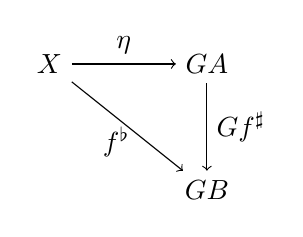
\begin{tikzpicture}[x=1cm, y=0.8cm]
            \node  (X) at (0, 2) {$X$};
            \node (F2) at (2, 2) {$GA$};s
            \node (F0) at (2, 0) {$GB$};
            \draw[->]  (X)  -- node[below, pos=0.4] {$f^\flat$} (F0);
            \draw[->]  (X)  -- node[above] {$\eta$} (F2);
            \draw[->] (F2)  -- node[right] {$Gf^\sharp$} (F0);
        \end{tikzpicture}
        \end{center}
    \end{enumerate}
    The morphism $\eta:X\to GA$ is called a \textbf{universal morphism}.
\end{property}
\begin{proof}
    $\int\hom_\mathcal{C}(X, G-)\cong\Delta  X\downarrow G$.
\end{proof}

\section{Adjunctions}

\subsection{Adjunct Functors}

Again, we do not distinguish between $F:\mathcal{C}^{op}\to\mathcal{D}^{op}$ and $F:\mathcal{C}\to\mathcal{D}$ here.

\begin{definition}
    Given a bijection $\hom_\mathcal{D}(FX, A)\cong\hom_\mathcal{C}(X, GA)$.
    Each pair of morphisms $$f^\sharp:FX\to A\qquad\leftrightarrows\qquad f^\flat:X\to GA$$ in the hom-sets are said to be \textbf{adjunct} of each other.
\end{definition}

\begin{definition}
    Two functors $F:\mathcal{C}^{op}\to\mathcal{D}^{op}$ and $G:\mathcal{D}\to\mathcal{C}$ be are said to be \textbf{adjoint} if the two bifunctors
    \[
        \hom_\mathcal{D}(F-, -)\cong \hom_\mathcal{C}(-, G-)
    \]
    are isomorphic in $[\mathcal{C}^{op}\times\mathcal{D}, \textbf{Set}]$, denoted as $F\dashv G$.
        \begin{center}
        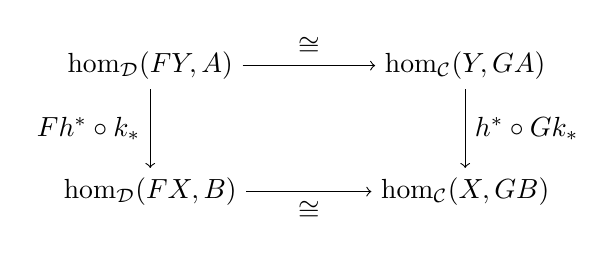
\begin{tikzpicture}[x=1cm, y=0.8cm]
            \node (FXY)  at (0, 2) {$\hom_\mathcal{D}(FY, A)$};
            \node (FXB) at (0, 0) {$\hom_\mathcal{D}(FX, B)$};
            \node (XGY)  at (4, 2) {$\hom_\mathcal{C}(Y, GA)$};
            \node (XGB) at (4, 0) {$\hom_\mathcal{C}(X, GB)$};
            \draw[->] (FXY)  -- node[above] {$\cong$} (XGY);
            \draw[->] (FXB) -- node[below] {$\cong$} (XGB);
            \draw[->] (FXY)  -- node[left ] {$Fh^*\circ k_*$} (FXB);
            \draw[->] (XGY)  -- node[right] {$h^*\circ Gk_*$} (XGB);
        \end{tikzpicture}
        \end{center}
    In this case, we said $F$ is left adjoint to $G$ and $G$ is right adjoint to $F$.
\end{definition}

\begin{definition}
    Let $F:\mathcal{C}\leftrightarrows\mathcal{D}:G$ be a pair of functors, $\eta:1_\mathcal{C}\Rightarrow GF$ and $\epsilon:FG\Rightarrow 1_\mathcal{D}$ be natural transformations.
    If the \textbf{triangle identities} hold:
    \begin{center}
    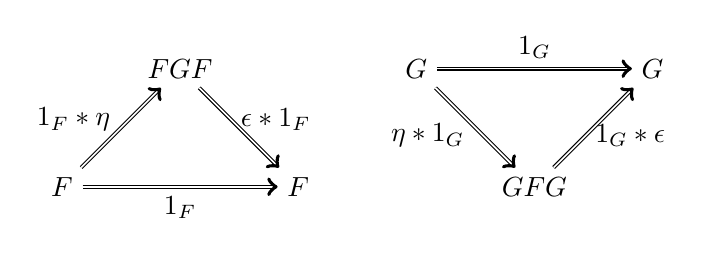
\begin{tikzpicture}[x=1.5cm, y=1.5cm]
        \node (F0)  at (0, 0) {$F$};
        \node (F2)  at (2, 0) {$F$};
        \node (FGF) at (1, 1) {$FGF$};
        \node (G3)  at (3, 1) {$G$};
        \node (G5)  at (5, 1) {$G$};
        \node (GFG) at (4, 0) {$GFG$};
        \draw[->,double] (F0)  -- node[below] {$1_F$} (F2);
        \draw[->,double] (F0)  -- node[ left, pos=0.6] {$1_F*\eta\ $} (FGF);
        \draw[->,double] (FGF) -- node[right, pos=0.4] {$\epsilon*1_F$} (F2);
        \draw[->,double] (G3)  -- node[above] {$1_G$} (G5);
        \draw[->,double] (G3)  -- node[ left, pos=0.6] {$\eta*1_G\ $} (GFG);
        \draw[->,double] (GFG) -- node[right, pos=0.4] {$1_G*\epsilon$} (G5);
    \end{tikzpicture}
    \end{center}
    then $\eta:1_\mathcal{C}\Rightarrow GF$ is called the \textbf{unit}, and $\epsilon:FG\Rightarrow 1_\mathcal{D}$ is called the \textbf{counit}.
\end{definition}

Note that for every object $X$,
\[
    (1_F*\eta)_X = F\eta_X, \
    (\epsilon*1_F)_X = \epsilon_{FX},\
    (\eta*1_G)_X = \eta_{GX}, \
    (1_G*\epsilon)_X = G\epsilon_X;
\]
we may write $1_F*\eta$ as $F\eta$ for short.

\begin{theorem}
    The following are equivalent:
    \begin{enumerate}
        \item There is a natural isomorphism $\hom_\mathcal{D}(F-, -)\cong\hom_\mathcal{C}(-, G-)$.
        \item The universal property $\hom_\mathcal{D}(A_X, -)\cong\hom_\mathcal{C}(X, G-)$ holds for all $X$.
        \item The unit $\eta:1_\mathcal{C}\Rightarrow GF$ and the counit $\epsilon:FG\Rightarrow 1_\mathcal{D}$ exist.
        \item The left diagram commute iff the right diagram commute:
        \begin{center}
        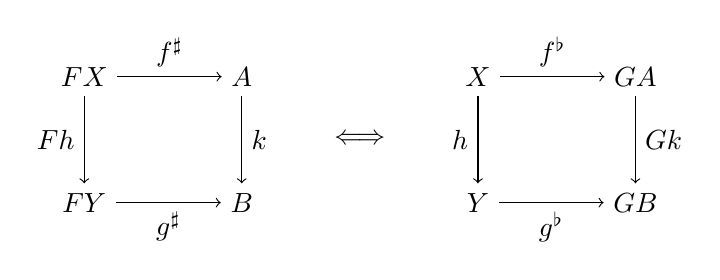
\begin{tikzpicture}[x=1cm, y=0.8cm]
            \node (FY) at (0, 0) {$FY$};
            \node (FX)  at (0, 2) {$FX$};
            \node (B)  at (2, 0) {$B$};
            \node (A)   at (2, 2) {$A$};
            \node (iff) at (3.5, 1) {$\iff$};
            \node (GB) at (7, 0) {$GB$};
            \node (GA)  at (7, 2) {$GA$};
            \node (Y)  at (5, 0) {$Y$};
            \node (X)   at (5, 2) {$X$};
            \draw[->] (FX)  -- node[above] {$f^\sharp$} (A);
            \draw[->] (FX)  -- node[ left] {$Fh$} (FY);
            \draw[->] (FY) -- node[below] {$g^\sharp$} (B);
            \draw[->] (A)   -- node[right] {$k$} (B);
            \draw[->] (X)  -- node[above] {$f^\flat$} (GA);
            \draw[->] (X)  -- node[ left] {$h$} (Y);
            \draw[->] (Y) -- node[below] {$g^\flat$} (GB);
            \draw[->] (GA)   -- node[right] {$Gk$} (GB);
        \end{tikzpicture}
        \end{center}
    \end{enumerate}
\end{theorem}
\begin{proof}    

    $(2)\Rightarrow(1)$.
    Since the Yoneda embedding $y$ is fully faithful, for each $h:X\to Y$, there exists a unique morphism $A_h:A_{X}\to A_{Y}$ such that the diagram commute:
    \begin{center}
    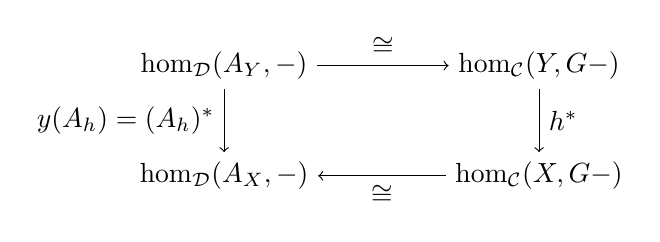
\begin{tikzpicture}[x=2cm, y=0.7cm]
        \node (AX)  at (0, 2) {$\hom_\mathcal{D}(A_{Y}, -)$};
        \node (AY) at (0, 0) {$\hom_\mathcal{D}(A_X, -)$};
        \node (X)   at (2, 2) {$\hom_\mathcal{C}(Y, G-)$};
        \node (Y)  at (2, 0) {$\hom_\mathcal{C}(X, G-)$};
        \draw[->] (AX)  -- node[above] {$\cong$} (X);
        \draw[<-] (AY) -- node[below] {$\cong$} (Y);
        \draw[->] (X)   -- node[right] {$h^*$} (Y);
        \draw[->] (AX)  -- node[ left] {$y(A_h)=(A_h)^*$} (AY);
    \end{tikzpicture}
    \end{center}
    Then $F:\mathcal{C}\to\mathcal{D}:X\mapsto A_X:h\mapsto A_h$ is the functor such that $F\dashv G$.
    
    % $(1)\Rightarrow(3)$.
    % Define $\eta:1_\mathcal{C}\Rightarrow GF$ and $\epsilon:FG\Rightarrow 1_\mathcal{D}$ by
    % \begin{center}
    % \begin{tikzpicture}[x=0.5cm, y=0.7cm]
    %     \node at (0, 1) {$\hom_\mathcal{D}(FX, FX)$};
    %     \node at (3.5, 1) {$\cong$};
    %     \node at (7, 1) {$\hom_\mathcal{C}(X, GFX)$};
    %     \node at (14, 1) {$\hom_\mathcal{D}(FGY, Y)$};
    %     \node at (17.5, 1) {$\cong$};
    %     \node at (21, 1) {$\hom_\mathcal{C}(GY, GY)$};
    %     \node at (0, 0) {$1_{FX}$};
    %     \node at (3.5, 0) {$\leftrightarrows$};
    %     \node at (7, 0) {$\eta_X=1_{FX}^\flat$};
    %     \node at (14, 0) {$\epsilon_Y=1_{GY}^\sharp$};
    %     \node at (17.5, 0) {$\leftrightarrows$};
    %     \node at (21, 0) {$1_{GY}$};
    % \end{tikzpicture}
    % \end{center}
    % By (4), the following diagrams commute:
    % \begin{center}
    % \begin{tikzpicture}[x=1cm, y=0.8cm]
    %     \node (FY) at (-1.5, 4) {$FY$};
    %     \node (FX)  at (-1.5, 2) {$FX$};
    %     \node (FGF) at (-1.5, 0) {$FGFX$};
    %     \node (B)  at (1.5, 4) {$FY$};
    %     \node (Y)   at (1.5, 2) {$FX$};
    %     \node (FX2) at (1.5, 0) {$FX$};
    %     \node (iff) at (3.6, 1) {$\iff$};
    %     \node (iff) at (3.6, 3) {$\iff$};
    %     \node (iff) at (3.6, 3.6) {Naturality};
    %     \node (iff) at (3.6, 1.6) {Triangle};
    %     \node (GB) at (8.5, 4) {$GFY$};
    %     \node (GY)  at (8.5, 2) {$GFX$};
    %     \node (GF8) at (8.5, 0) {$GFX$};
    %     \node (Y)  at (5.5, 4) {$Y$};
    %     \node (X)   at (5.5, 2) {$X$};
    %     \node (GF5) at (5.5, 0) {$GFX$};
    %     \draw[->] (FX)  -- node[above] {$1_{FX}$} (Y);
    %     \draw[->] (FGF)  -- node[above] {$\epsilon_{FX}$} (FX2);
    %     \draw[->] (FX)  -- node[ left] {$Ff$} (FY);
    %     \draw[->] (FX)  -- node[ left] {$F\eta_X$} (FGF);
    %     \draw[->] (FY) -- node[above] {$1_{FY}$} (B);
    %     \draw[->] (Y)   -- node[right] {$Ff$} (B);
    %     \draw[->] (Y)   -- node[right] {$1_{FX}$} (FX2);
    %     \draw[->] (X)  -- node[above] {$\eta_X$} (GY);
    %     \draw[->] (X)  -- node[ left] {$f$} (Y);
    %     \draw[->] (X)  -- node[ left] {$\eta_X$} (GF5);
    %     \draw[->] (GF5) -- node[above] {$1_{GFX}$} (GF8);
    %     \draw[->] (Y)  -- node[above] {$\eta_{Y}$} (GB);
    %     \draw[->] (GY)   -- node[right] {$GFf$} (GB);
    %     \draw[->] (GY)   -- node[right] {$1_{GFX}$} (GF8);
    % \end{tikzpicture}
    % \end{center}

    $(3)\Rightarrow(1)$.
    Given unit $\eta$ and counit $\epsilon$.
    The transformation $\hom_\mathcal{D}(F-, -)\Rightarrow\hom_\mathcal{C}(-, G-)$ is determined by
    \begin{center}
    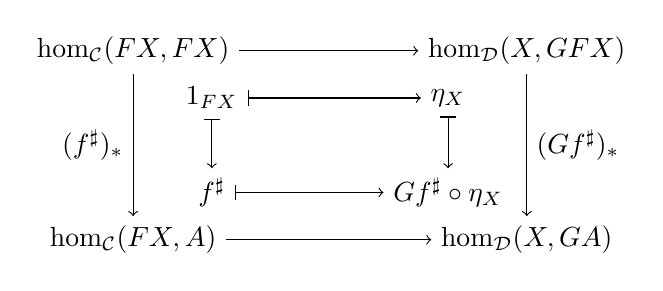
\begin{tikzpicture}[x=1cm, y=0.6cm]
        \node (1x)  at (1, 3) {$1_{FX}$};
        \node (f)   at (1, 1) {$f^\sharp$};
        \node (a1)  at (4, 3) {$\eta_X$};
        \node (aAf) at (4, 1) {$Gf^\sharp\circ\eta_X$};
        \node (hxX) at (0, 4) {$\hom_\mathcal{C}(FX, FX)$};
        \node (hxY) at (0, 0) {$\hom_\mathcal{C}(FX, A)$};
        \node (FX)  at (5, 4) {$\hom_\mathcal{D}(X, GFX)$};
        \node (FY)  at (5, 0) {$\hom_\mathcal{D}(X, GA)$};
        \draw[->] (hxX) -- node[left]  {$(f^\sharp)_*$} (hxY);
        \draw[->] (FX)  -- node[right] {$(Gf^\sharp)_*$}     (FY);
        \draw[->] (hxX) -- node[above] {}  (FX);
        \draw[->] (hxY) -- node[below] {}  (FY);
        \draw[|->] (1x) --  (a1);
        \draw[|->] (1x) --  (f);
        \draw[|->] (a1) --  (aAf);
        \draw[|->] (f)  --  (aAf);
    \end{tikzpicture}
    \end{center}
    The bijection $\hom_\mathcal{D}(FX, A)\cong\hom_\mathcal{C}(X, GA)$ is given by
    \[
        f^\sharp\mapsto Gf^\sharp\circ\eta_X
        \quad\text{and}\quad
        f^\flat\mapsto\epsilon_A\circ Ff^\flat.
    \]

    $(1)\Rightarrow(3)$.
    Let $h:X\to Y$.
    By the dual version of Yoneda Lemma,
    \begin{center}
    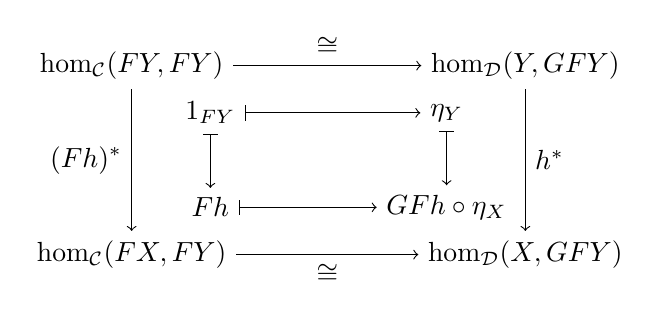
\begin{tikzpicture}[x=1cm, y=0.6cm]
        \node (1x)  at (1, 3) {$1_{FY}$};
        \node (f)   at (1, 1) {$Fh$};
        \node (a1)  at (4, 3) {$\eta_Y$};
        \node (aAf) at (4, 1) {$GFh\circ\eta_X$};
        \node (hxX) at (0, 4) {$\hom_\mathcal{C}(FY, FY)$};
        \node (hxY) at (0, 0) {$\hom_\mathcal{C}(FX, FY)$};
        \node (FX)  at (5, 4) {$\hom_\mathcal{D}(Y, GFY)$};
        \node (FY)  at (5, 0) {$\hom_\mathcal{D}(X, GFY)$};
        \draw[->] (hxX) -- node[left]  {$(Fh)^*$} (hxY);
        \draw[->] (FX)  -- node[right] {$h^*$}     (FY);
        \draw[->] (hxX) -- node[above] {$\cong$}  (FX);
        \draw[->] (hxY) -- node[below] {$\cong$}  (FY);
        \draw[|->] (1x) --  (a1);
        \draw[|->] (1x) --  (f);
        \draw[|->] (a1) --  (aAf);
        \draw[|->] (f)  --  (aAf);
    \end{tikzpicture}
    \end{center}
    % \[
    %     (Fh)^\flat = GFh\circ\eta_X = \hom_\mathcal{C}(h, GFY)(1_{FY}^\flat) = h^*(\eta_Y)=\eta_Y\circ h.
    % \]
    This proves the naturality of $\eta$, and the triangle identity is proved by
    \[
        1_{FX} 
        = \epsilon_{FX}\circ F(1_{FX}^\flat) 
        = \epsilon_{FX}\circ F(G1_{FX}\circ \eta_X)
        = \epsilon_{FX}\circ F\eta_X.
    \]
    
    
    $(1)\Rightarrow(4)$.
    Consider the correspondence:
    \begin{center}
    \begin{tabular}{ccc}
        $\hom_\mathcal{D}(FX, B)$ & $\cong$ & $\hom_\mathcal{C}(X, GB)$ \\[2pt]
        $k\circ f^\sharp$ & $\leftrightarrows$ & $Gk\circ f^\flat$ \\[2pt]
        $g^\sharp\circ Fh$ & $\leftrightarrows$ & $g^\flat\circ h$
    \end{tabular} 
    \end{center}

    $(4)\Rightarrow(1)$.
    Let $\phi^\sharp:FX\to A$ and $\phi^\flat:X\to GA$, then
        \begin{center}
        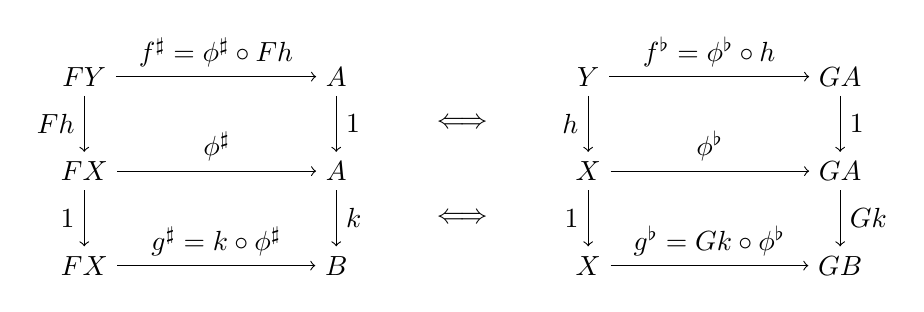
\begin{tikzpicture}[x=1.6cm, y=0.6cm]
            \node (FX0) at (0, 0) {$FX$};
            \node (FX2) at (0, 2) {$FX$};
            \node (FX4) at (0, 4) {$FY$};
            \node (Y0)  at (2, 0) {$B$};
            \node (Y2)  at (2, 2) {$A$};
            \node (Y4)  at (2, 4) {$A$};
            \node (X0) at (4, 0) {$X$};
            \node (X2) at (4, 2) {$X$};
            \node (X4) at (4, 4) {$Y$};
            \node (GY0)  at (6, 0) {$GB$};
            \node (GY2)  at (6, 2) {$GA$};
            \node (GY4)  at (6, 4) {$GA$};
            \node (iff) at (3, 1) {$\iff$};
            \node (iff) at (3, 3) {$\iff$};
            \draw[->] (FX4) -- node[above] {$f^\sharp=\phi^\sharp\circ Fh$} (Y4);
            \draw[->] (FX4) -- node[ left] {$Fh$} (FX2);
            \draw[->] (Y4)  -- node[right] {$1$} (Y2);
            \draw[->] (X4)  -- node[above] {$f^\flat=\phi^\flat\circ h$} (GY4);
            \draw[->] (X4)  -- node[ left] {$h$} (X2);
            \draw[->] (GY4)  -- node[right] {$1$} (GY2);
            \draw[->] (FX2) -- node[above] {$\phi^\sharp$} (Y2);
            \draw[->] (FX2) -- node[ left] {$1$} (FX0);
            \draw[->] (Y2)  -- node[right] {$k$} (Y0);
            \draw[->] (X2)  -- node[above] {$\phi^\flat$} (GY2);
            \draw[->] (X2)  -- node[ left] {$1$} (X0);
            \draw[->] (GY2)  -- node[right] {$Gk$} (GY0);
            \draw[->] (FX0) -- node[above] {$g^\sharp=k\circ\phi^\sharp$} (Y0);
            \draw[->] (X0)  edge node[above] {$g^\flat=Gk\circ\phi^\flat$} (GY0);
        \end{tikzpicture}
        \end{center}
\end{proof}

We called $(F, G, \eta, \epsilon):\mathcal{C}\to\mathcal{D}$ or $F\dashv G$ an \textbf{adjunction}.

\begin{property}
    Let $F\dashv G$ be an adjunction.
    The diagrams commute:
    \begin{center}
    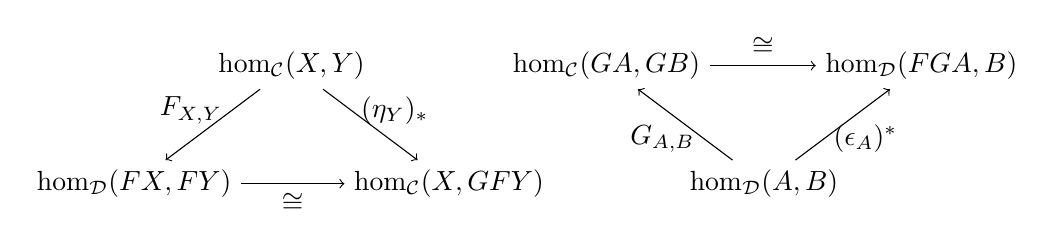
\begin{tikzpicture}[x=2cm, y=1.5cm]
        \node (00) at (0, 0) {$\hom_\mathcal{D}(FX, FY)$};
        \node (20) at (2, 0) {$\hom_\mathcal{C}(X, GFY)$};
        \node (11) at (1, 1) {$\hom_\mathcal{C}(X, Y)$};
        \draw[->] (00) -- node[below] {$\cong$} (20);
        \draw[->] (11) -- node[ left, pos=0.3] {$F_{X, Y}$} (00);
        \draw[->] (11) -- node[right, pos=0.3] {$(\eta_Y)_*$} (20);
        \node (30) at (3, 1) {$\hom_\mathcal{C}(GA, GB)$};
        \node (50) at (5, 1) {$\hom_\mathcal{D}(FGA, B)$};
        \node (41) at (4, 0) {$\hom_\mathcal{D}(A, B)$};
        \draw[->] (30) -- node[above] {$\cong$} (50);
        \draw[->] (41) -- node[ left, pos=0.3] {$G_{A, B}$} (30);
        \draw[->] (41) -- node[right, pos=0.3] {$(\epsilon_A)^*$} (50);
    \end{tikzpicture}
    \end{center}
\end{property}
\begin{proof}
    Let $h:X\to Y$.
    By Yoneda Lemma,
    \begin{center}
    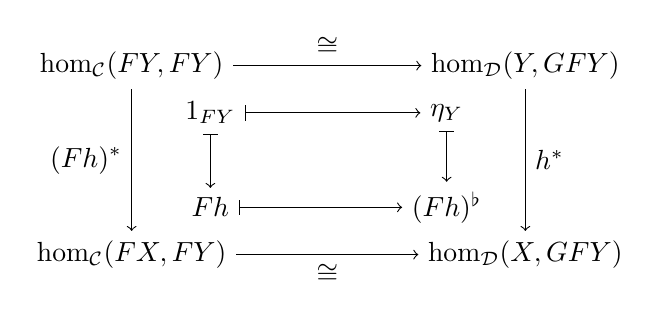
\begin{tikzpicture}[x=1cm, y=0.6cm]
        \node (1x)  at (1, 3) {$1_{FY}$};
        \node (f)   at (1, 1) {$Fh$};
        \node (a1)  at (4, 3) {$\eta_Y$};
        \node (aAf) at (4, 1) {$(Fh)^\flat$};
        \node (hxX) at (0, 4) {$\hom_\mathcal{C}(FY, FY)$};
        \node (hxY) at (0, 0) {$\hom_\mathcal{C}(FX, FY)$};
        \node (FX)  at (5, 4) {$\hom_\mathcal{D}(Y, GFY)$};
        \node (FY)  at (5, 0) {$\hom_\mathcal{D}(X, GFY)$};
        \draw[->] (hxX) -- node[left]  {$(Fh)^*$} (hxY);
        \draw[->] (FX)  -- node[right] {$h^*$}     (FY);
        \draw[->] (hxX) -- node[above] {$\cong$}  (FX);
        \draw[->] (hxY) -- node[below] {$\cong$}  (FY);
        \draw[|->] (1x) --  (a1);
        \draw[|->] (1x) --  (f);
        \draw[|->] (a1) --  (aAf);
        \draw[|->] (f)  --  (aAf);
    \end{tikzpicture}
    \end{center}
\end{proof}

\begin{corollary}
    Let $(F, G, \eta, \epsilon)$ be an adjunction.
    \begin{enumerate}
        \item $F$ is faithful $\iff$ every component of $\eta$ is monic.
        \item $F$ is full $\iff$ every component of $\eta$ is epic.
    \end{enumerate}
    Dually, 
    \begin{enumerate}
        \item $G$ is faithful $\iff$ every component of $\epsilon$ is epic.
        \item $G$ is full $\iff$ every component of $\epsilon$ is monic.
    \end{enumerate}
\end{corollary}
\begin{proof}
    $\eta_Y$ is monic $\iff(\eta_Y)_*$ is injective $\iff F_{X, Y}$ is injective.
\end{proof}

\subsection{The Calculus of adjunctions}

\begin{property}
\label{calculus of adjunction}
    Let $(F, G, \eta, \epsilon):\mathcal{C}\to\mathcal{D}$ be an adjunction.
    \begin{enumerate}
        \item Let $(F', G', \eta', \epsilon'):\mathcal{D}\to\mathcal{E}$ be an adjunction.
        There is an adjunction
        \[
            (F'F, GG', G\eta'F\circ\eta, \epsilon'\circ F'\epsilon G'):\mathcal{C}\to\mathcal{E}
        \]
        \item If $F'\dashv G$, there exists $\theta:F\cong F'$ such that the diagrams commute:
        \begin{center}
        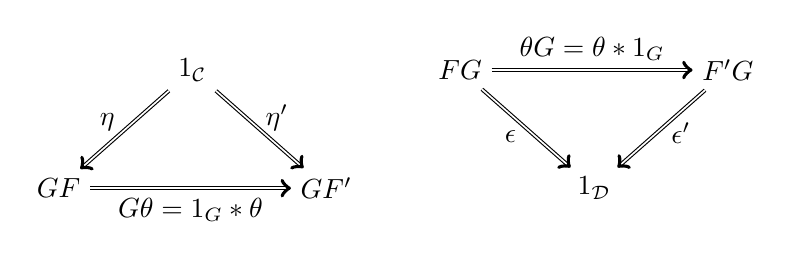
\begin{tikzpicture}[x=1.7cm, y=1.5cm]
            \node (GF0) at (0, 0) {$GF$};
            \node (GF2) at (2, 0) {$GF'$};
            \node (1C)  at (1, 1) {$1_\mathcal{C}$};
            \node (FG3) at (3, 1) {$FG$};
            \node (FG5) at (5, 1) {$F'G$};
            \node (1D)  at (4, 0) {$1_\mathcal{D}$};
            \draw[->,double] (GF0) -- node[below] {$G\theta=1_G*\theta$} (GF2);
            \draw[->,double] (1C)  -- node[right, pos=0.35] {$\ \eta'$} (GF2);
            \draw[->,double] (1C)  -- node[ left, pos=0.4] {$\eta\ $} (GF0);
            \draw[->,double] (FG3) -- node[above] {$\theta G=\theta*1_G$} (FG5);
            \draw[->,double] (FG3)  -- node[ left, pos=0.6] {$\epsilon\ $} (1D);
            \draw[->,double] (FG5)  -- node[right, pos=0.55] {$\,\epsilon'$} (1D);
        \end{tikzpicture}
        \end{center}
    \end{enumerate}
\end{property}
\begin{proof}
    (1).
    The isomorphism
    \[
        \hom_\mathcal{E}(F'F-, -)\cong\hom_\mathcal{D}(F-, G'-)\cong\hom_\mathcal{C}(-, GG'-),
    \]
    maps $1_{F'FX}$ to $G\eta'_{FX}\circ\eta_X$.
    
    (2).
    Define $\theta:F\Rightarrow F'$ and $\theta':F'\Rightarrow F$ by
    \begin{center}
    \begin{tabular}{ccccc}
        $\hom_\mathcal{D}(FX, F'X)$ & $\cong$ & $\hom_\mathcal{C}(X, GF'X)$ & $\cong$ & $\hom_\mathcal{D}(F'X, F'X)$ \\[2pt]
        $\theta_X=\epsilon_{F'X}\circ F\eta'_X$ & $\leftrightarrows$ & $\eta'_X$ & $\leftrightarrows$ & $1_{F'X}$ \\[5pt]
        $\hom_\mathcal{D}(FX, FX)$ & $\cong$ & $\hom_\mathcal{C}(X, GFX)$ & $\cong$ & $\hom_\mathcal{D}(F'X, FX)$ \\[2pt]
        $1_{FX}$ & $\leftrightarrows$ & $\eta_X$ & $\leftrightarrows$ & $\theta'_X=\epsilon'_{FX}\circ F'\eta_X$
    \end{tabular}
    \end{center}
    Then the diagram commute:
    \begin{center}
    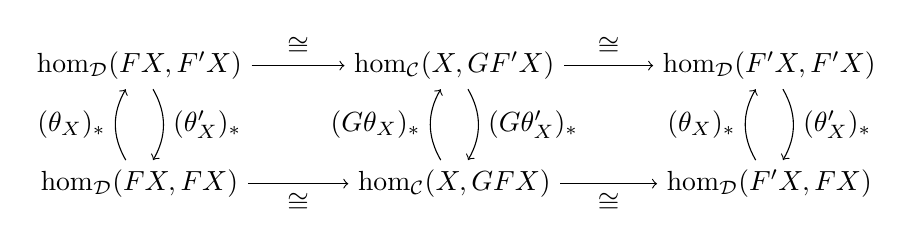
\begin{tikzpicture}[x=2cm, y=1.5cm]
        \node (00) at (0, 0) {$\hom_\mathcal{D}(FX, FX)$};
        \node (01) at (0, 1) {$\hom_\mathcal{D}(FX, F'X)$};
        \node (10) at (2, 0) {$\hom_\mathcal{C}(X, GFX)$};
        \node (11) at (2, 1) {$\hom_\mathcal{C}(X, GF'X)$};
        \node (20) at (4, 0) {$\hom_\mathcal{D}(F'X, FX)$};
        \node (21) at (4, 1) {$\hom_\mathcal{D}(F'X, F'X)$};
        \draw[->] (00) -- node[below] {$\cong$} (10);
        \draw[->] (10) -- node[below] {$\cong$} (20);
        \draw[->] (01) -- node[above] {$\cong$} (11);
        \draw[->] (11) -- node[above] {$\cong$} (21);
        \draw[<-,bend right] (01) edge node[ left] {$(\theta_X)_*$} (00);
        \draw[<-,bend right] (11) edge node[ left] {$(G\theta_X)_*$} (10);
        \draw[<-,bend right] (21) edge node[ left] {$(\theta_X)_*$} (20);
        \draw[->,bend  left] (01) edge node[right] {$(\theta'_X)_*$} (00);
        \draw[->,bend  left] (11) edge node[right] {$(G\theta'_X)_*$} (10);
        \draw[->,bend  left] (21) edge node[right] {$(\theta'_X)_*$} (20);
    \end{tikzpicture}
    \end{center}
    Thus $(\theta_X)_*(\theta'_X)=\theta_X\circ\theta'_X=1_{F'X}$ and $(G\theta_X)_*(\eta_X)=G\theta_X\circ\eta_X=\eta'_X$.
\end{proof}

\subsection{Equivalence}

An isomorphism consists of morphisms $f:X\leftrightarrows Y:g$ with
\[
    1_X=gf
    \quad\text{and}\quad
    fg=1_Y.
\]
The equivalence is the higher notion of isomorphism.

\begin{definition}
    Let $\mathcal{C}$ and $\mathcal{D}$ be categories.
    \begin{enumerate}
        \item An \textbf{equivalence} consist of functors $F:\mathcal{C}\leftrightarrows\mathcal{D}:G$ with
        \[
            \eta:1_\mathcal{C}\cong GF
            \quad\text{ and }\quad
            \rho:FG\cong 1_\mathcal{D}.
        \]
        \item The equivalence is called an \textbf{adjoint equivalence} if $$(F, G, \eta, \rho):\mathcal{C}\to\mathcal{D}$$is an adjunction.
    \end{enumerate}
\end{definition}

Equivalence defines an equivalence relation on \textbf{Cat}.

\begin{lemma}
    Let $F:\mathcal{C}\leftrightarrows\mathcal{D}:G$ be an equivalence.
    \begin{enumerate}
        \item If $(F, G, \eta, \rho):\mathcal{C}\to\mathcal{D}$ is an adjoint equivalence, so is $(G, F, \rho^{-1}, \eta^{-1})$.
        \item The left diagram commute iff the right diagram commute:
        \begin{center}
        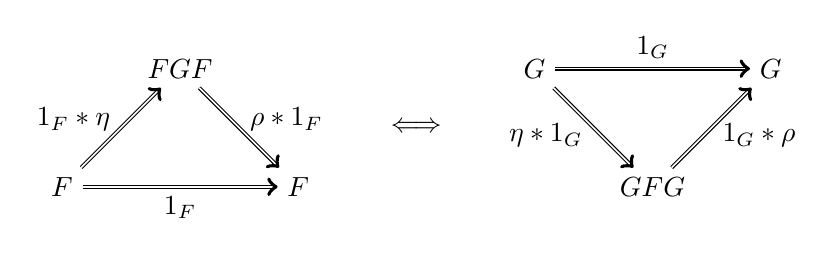
\begin{tikzpicture}[x=1.5cm, y=1.5cm]
            \node (F0)  at (0, 0) {$F$};
            \node (F2)  at (2, 0) {$F$};
            \node (FGF) at (1, 1) {$FGF$};
            \node (G3)  at (4, 1) {$G$};
            \node (iff)  at (3, 0.5) {$\iff$};
            \node (G5)  at (6, 1) {$G$};
            \node (GFG) at (5, 0) {$GFG$};
            \draw[->,double] (F0)  -- node[below] {$1_F$} (F2);
            \draw[->,double] (F0)  -- node[ left, pos=0.6] {$1_F*\eta\ $} (FGF);
            \draw[->,double] (FGF) -- node[right, pos=0.4] {$\ \rho*1_F$} (F2);
            \draw[->,double] (G3)  -- node[above] {$1_G$} (G5);
            \draw[->,double] (G3)  -- node[ left, pos=0.6] {$\eta*1_G\ $} (GFG);
            \draw[->,double] (GFG) -- node[right, pos=0.4] {$\ 1_G*\rho$} (G5);
        \end{tikzpicture}
        \end{center}
    \end{enumerate}
\end{lemma}
\begin{proof}
    (2).
    Suppose that $\rho F\circ F\eta=1_F=F\eta^{-1}\circ\epsilon^{-1}F$.
    By the naturality of $G\rho^{-1}:G\cong GFG$, we have
    \begin{align*}
        G\rho \circ \eta G
        & = G\rho \circ G1_FG \circ \eta G
          = G\rho \circ GF\eta^{-1}G \circ G\rho^{-1}FG \circ \eta G \\
        & = G\rho \circ G\rho^{-1} \circ \eta^{-1}G \circ \eta G
          = 1_G.
    \end{align*}
\end{proof}

\begin{definition}
    Let $F:\mathcal{C}\to\mathcal{D}$ be a functor.
    \begin{enumerate}
        \item $F$ is said to be \textbf{essentially injective} if $FX\cong FY$ implies $X\cong Y$.
        \item $F$ is said to be \textbf{essentially surjective} if for all $A\in\ob\mathcal{D}$, there exists $X\in\ob\mathcal{C}$ such that $A\cong FX$.
    \end{enumerate}
\end{definition}

Up to isomorphism, an essentially injective functor is injective on objects.

\begin{definition}
    A \textbf{skeleton} of $\mathcal{C}$ is a skeletal full subcategory $sk\mathcal{C}$ of $\mathcal{C}$.
\end{definition}

% It fails to define a functor $sk(-):\textbf{Cat}\to\textbf{Cat}$ since $sk(G\circ F)$ may \textbf{not} be equal to $sk G\circ skF$.
% It is just a pseudofunctor.

\begin{property}
    Let $F:\mathcal{C}\to\mathcal{D}$ be a functor.
    \begin{enumerate}
        \item Fully faithful functors are essentially injective.
        \item Every category has a skeleton.
    \end{enumerate}
\end{property}
\begin{proof}
    (2).
    Taking one object in each isomorphism class in $\mathcal{C}$, then the full subcategory on this collection of objects is a skeleton of $\mathcal{C}$.
\end{proof}

\begin{theorem}
    The following are equivalent:
    \begin{enumerate}
        \item $F:\mathcal{C}\leftrightarrows\mathcal{D}:G$ is an equivalence.
        \item There is an adjoint equivalence $(F, G, \eta, \epsilon):\mathcal{C}\to\mathcal{D}$.
        \item $F:\mathcal{C}\to\mathcal{D}$ is a fully faithful and essentially surjective functor.
        \item $sk\mathcal{C}\cong sk\mathcal{D}$.
    \end{enumerate}
\end{theorem}
\begin{proof}
    $(1)\Rightarrow(2)$.
    Let $\eta:1_\mathcal{C}\cong GF$ and $\rho:FG\cong1_\mathcal{D}$.
    Then the function
    \[
        \hom_\mathcal{C}(GA, GA) 
        \to
        \hom_\mathcal{D}(FGA, A)
        \to
        \hom_\mathcal{D}(GA, GA)
    \]
    maps $1_{GA}$ to $G(\rho_A\circ F1_{GA})\circ\eta_X=G\rho_A\circ\eta_{GA}$.
    Define $\gamma=G\rho\circ\eta G$ and
    \[
        \epsilon = \rho\circ F\gamma^{-1} = \rho\circ F\eta^{-1}G\circ FG\rho^{-1},
    \]
    then by the naturality of $\eta$,
    \[
        G\epsilon \circ \eta_G
        = G\rho \circ GF\gamma^{-1} \circ \eta G
        = G\rho \circ \eta G \circ \gamma^{-1}
        = 1_G
    \]
    and by the naturality of $F\eta^{-1}:FGF\cong F$,
    \[
        \epsilon F \circ F\eta 
        = \rho F \circ F\eta^{-1}GF \circ FG\rho^{-1}F \circ F\eta 
        = \rho F\circ \rho^{-1}F \circ F\eta^{-1} \circ F\eta
        = 1_F.
    \]
    
    $(2)\Rightarrow(3)$.
    Since $\eta:1_\mathcal{C}\cong GF$ is a natural isomorphism, $F$ is fully faithful.
    Since $\epsilon_A:FGA\cong A$ for all $A\in\ob\mathcal{D}$, $F$ is essentially surjective.

    $(3)\Rightarrow(2)$.
    For each $A\in\ob\mathcal{D}$, choose $GA\in\ob\mathcal{C}$ with $\epsilon_A:FGA\cong A$ since $F$ is essentially surjective.
    For each morphism $f:A\to B$ in $\mathcal{D}$, there is a unique $Gf:GA\to GB$ such that $FGf=\epsilon^{-1}_B\circ f\circ\epsilon_A$ since $F$ is fully faithful.
    Hence $G:\mathcal{D}\to\mathcal{C}$ is a functor with $\epsilon:FG\cong1_\mathcal{D}$, and $\eta_X:X\cong GFX$ is defined by the unique isomorphism such that $F\eta_X=(\epsilon_{FX})^{-1}$.

    $(3)\Rightarrow(4)$.
    Since the inclusion $i_\mathcal{C}:sk\mathcal{C}\to\mathcal{C}$ is fully faithful and essentially surjective, we have an equivalence $i_\mathcal{C}:sk\mathcal{C}\leftrightarrows\mathcal{C}:r_\mathcal{C}$.
    By symmetry, $r_\mathcal{D}:\mathcal{D}\to sk\mathcal{D}$ is fully faithful and essentially surjective, so is $skF=r_\mathcal{D}\circ F\circ i_\mathcal{C}:sk\mathcal{C}\to sk\mathcal{D}$.
    Again, choose $\epsilon_A=1_A$ for all $A\in sk\mathcal{D}$, then the selected functor $G:sk\mathcal{D}\to sk\mathcal{C}$ from the proof of $(3)\Rightarrow(2)$ is the inverse of $skF$.
\end{proof}

\subsection{Terminology and Constructions}

\begin{definition}
    Let $\mathcal{D}$ be a full subcategory of $\mathcal{C}$ with $r\dashv i$.
    \begin{enumerate}
        \item $r:\mathcal{C}\to\mathcal{D}$ is called the \textbf{reflector}.
        \item $i:\mathcal{D}\to\mathcal{C}$ is the inclusion functor.
        \item $r\dashv i$ is the \textbf{reflection-inclusion adjunction}.
    \end{enumerate}
\end{definition}

For example, the inclusion $i_\mathcal{C}:sk\mathcal{C}\to\mathcal{C}$ has a reflector $r_\mathcal{C}:\mathcal{C}\to sk\mathcal{C}$, which maps each object $X$ to the unique object $r_\mathcal{C}X$ in $sk\mathcal{C}$ that isomorphic to $X$.

\begin{definition}
    Let $U:\mathcal{D}\to\mathcal{C}$ be a faithful functor with $F\dashv U$.
    \begin{enumerate}
        \item $F:\mathcal{C}\to\mathcal{D}$ is said to be \textbf{free}.
        \item $U:\mathcal{D}\to\mathcal{C}$ is said to be \textbf{forgetful}.
        \item $F\dashv U$ is the \textbf{free-forgetful adjunction}.
    \end{enumerate}
\end{definition}

Let $U:\textbf{Cat}\to\textbf{Set}$ be the faithful functor that maps a category to the set of objects.
Then $U$ has a left adjoint $\textbf{Set}\to\textbf{Cat}$, which maps a set to the discrete category.

\begin{property}
    Let $U:\mathcal{D}\to\textbf{Set}$ be a forgetful functor.
    The following are equivalent:
    \begin{enumerate}
        \item All components of the unit $\eta:1_\textbf{Set}\Rightarrow UF$ are monic.
        \item $|UA|>1$ for some $A\in\ob\mathcal{D}$.
    \end{enumerate}
\end{property}
\begin{proof}
    If $\eta_X$ is not monic, then $\eta_X(x_1)=\eta_X(x_2)$ for some $x_1\ne x_2\in X$.
    Let $A\in\ob\mathcal{D}$ and $a_1, a_2\in UA$.
    Take $f^\flat:X\to UA$ such that $f^\flat(x_1)=a_1$ and $f^\flat(x_2)=a_2$, then $f^\flat=Uf^\sharp\circ\eta_X$ and hence
    \[
        a_1 = f^\flat(x_1) = (Uf^\sharp\circ\eta_X)(x_1) = (Uf^\sharp\circ\eta_X)(x_2) = f^\flat(x_2) = a_2.
    \]
    Therefore, $|UA|>1$ for some $A$ implies all $\eta_X$ are monic.
\end{proof}

\begin{definition}
    Let $\otimes$ and $[-, -]$ be functors with
    \[
        \hom_\mathcal{C}(-\otimes-, -) \cong \hom_\mathcal{C}(-, [-, -]).
    \]
    \begin{enumerate}
        \item $\otimes:\mathcal{C}\times\mathcal{C}\to\mathcal{C}$ is called \textbf{tensor}.
        \item $[-, -]:\mathcal{C}^{op}\times\mathcal{C}\to\mathcal{C}$ is called \textbf{internal hom}.
        \item $\otimes\dashv[-, -]$ is the \textbf{tensor-hom adjunction}.
    \end{enumerate}
\end{definition}

\begin{property}
    Recall $\mathcal{C}\times\mathcal{D}$ is the product of categories, and $[\mathcal{C}, \mathcal{D}]$ is the functor category.
    Then $\times\dashv[-, -]$ is a tensor-hom adjunction.
    Moreover, 
    \begin{center}
    \begin{tabular}{ccccc}
        $\hom_\textbf{Cat}(\mathcal{C}^{op}\times\mathcal{C}, \textbf{Set})$ & $\cong$ & $\hom_\textbf{Cat}(\mathcal{C}^{op}, [\mathcal{C}, \textbf{Set}])$ \\[2pt]
        Hom Functor & $\leftrightarrows$ & Yoneda Embedding
    \end{tabular}
    \end{center}
\end{property}
\begin{proof}
    The component
    \[
        \Phi:\hom_\textbf{Cat}(\mathcal{C}\times\mathcal{D}, \mathcal{E})\to\hom_\textbf{Cat}(\mathcal{C}, [\mathcal{D}, \mathcal{E}]):F\mapsto\Phi(F)
    \]
    of the isomorphism $\hom_\textbf{Cat}(-\times-, -)\cong\hom_\textbf{Cat}(-, [-, -])$ is defined by
    \[
        \Phi(F):\mathcal{C}\to[\mathcal{D}, \mathcal{E}]:
        X\mapsto F(X, -):f\mapsto F(f, -).
    \]
\end{proof}

\begin{definition}
    Let End be a functor with
    \[\textstyle
        \hom_\mathcal{D}(-, \int_\mathcal{C}-)\cong
        \hom_{[\mathcal{C}^{op}\times\mathcal{C}, \textbf{Set}]}(\hom_\mathcal{C}, \hom_\mathcal{D}(-, -))
    \]
    \begin{enumerate}
        \item $\int_\mathcal{C}:[\mathcal{C}^{op}\times\mathcal{C}, \mathcal{D}]\to\mathcal{D}$ is called \textbf{end}.
        \item $\hom_\mathcal{D}(-, -):\mathcal{D}^{op}\times[\mathcal{C}^{op}\times\mathcal{C}, \mathcal{D}]\to[\mathcal{C}^{op}\times\mathcal{C}, \textbf{Set}]:(X, F)\mapsto \hom_\mathcal{D}(X, F-)$.
    \end{enumerate}
\end{definition}

\subsection{Examples}

Recall that a poset $P$ is a skeletal category with
\[
    \hom_P(x, y) = \begin{cases}
        1 & x\le y \\
        0 & x\not\le y.
    \end{cases}
\]

\begin{definition}
    A \textbf{Galois connection} is an adjunction between posets.
\end{definition}

In other words, a Galois connection between posets $P$ and $Q$ consist of a pair of order-preserving functions $f:P\leftrightarrows Q:g$ such that
\[
    f(a) \le b \iff a \le g(b)
\]
for all $a\in P$ and $b\in Q$.

\section{Limits}

\subsection{Diagonal-Limit Adjunction}

\begin{definition}
    Let $F:\mathcal{J}\to\mathcal{C}$ be a functor.
    \begin{enumerate}
        \item The object $\lim F$ is called the \textbf{limit} of $F$ if
        \[
            \hom_{[\mathcal{J}, \mathcal{C}]}(\Delta-, F) \cong \hom_\mathcal{C}(-, \lim F).
        \]
        \item Dually, the object $\colim F$ is called the \textbf{colimit} of $F$ if
        \[
            \hom_{[\mathcal{J}^{op}, \mathcal{C}^{op}]}(F, \Delta-) \cong \hom_{\mathcal{C}^{op}}(\colim F, -).
        \]
    \item If all functor from $\mathcal{J}$ to $\mathcal{C}$ has a limit, then
        \[
            \hom_{[\mathcal{J}, \mathcal{C}]}(\Delta-, -) \cong \hom_\mathcal{C}(-, \lim -)
        \]
        is called the \textbf{diagonal-limit adjunction}.
    \end{enumerate}
\end{definition}

The colimit of $F:\mathcal{J}\to\mathcal{C}$ is the limit of $F^{op}:\mathcal{J}^{op}\to\mathcal{C}^{op}$.

\begin{definition}
    Let $F:\mathcal{J}\to\mathcal{C}$ be a functor with the limit $\lim F$.
    \begin{enumerate}
        \item A natural transformation from $\Delta X$ to $F$ is called a \textbf{cone} to $F$.
        \item The counit $\epsilon_F:\Delta\lim F\Rightarrow F$ is called the \textbf{limit cone}.
    \end{enumerate}
\end{definition}

Therefore, for every cone $\phi^\sharp:\Delta X\Rightarrow F$ and object $j\in\ob\mathcal{J}$, there exists a unique morphism $\phi^\flat:X\to \lim F$ such that the diagrams commute
\begin{center}
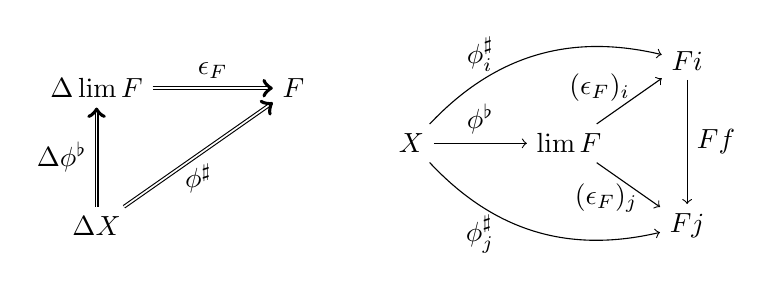
\begin{tikzpicture}[x=1cm, y=0.7cm]
    \node (Dlim) at (0, 2) {$\Delta\lim F$};
    \node (DX) at (0, -0.5) {$\Delta X$};
    \node (F) at (2.5, 2) {$F$};
    \draw[->,double] (DX)   -- node[below] {$\phi^\sharp$} (F);
    \draw[->,double] (Dlim) -- node[above] {$\epsilon_F$} (F);
    \draw[->,double] (DX)   -- node[ left] {$\Delta\phi^\flat$} (Dlim);
    \node (X)   at (4, 1) {$X$};
    \node (lim) at (6, 1) {$\lim F$};
    \node (Fi) at (7.5, 2.5) {$Fi$};
    \node (Fj) at (7.5,-0.5) {$Fj$};
    \draw[->] (X)   -- node[above] {$\phi^\flat$} (lim);
    \draw[->, bend left] (X)  edge node[above, pos=0.25] {$\phi^\sharp_i$} (Fi);
    \draw[->, bend right] (X)  edge node[below, pos=0.25] {$\phi^\sharp_j$} (Fj);
    \draw[->] (lim)   -- node[left, pos=0.8] {$(\epsilon_F)_i\ $} (Fi);
    \draw[->] (lim)   -- node[left, pos=0.8] {$(\epsilon_F)_j$} (Fj);
    \draw[->] (Fi) edge node[right] {$Ff$} (Fj);
\end{tikzpicture}
\end{center}
for all $f:i\to j$ in $\mathcal{J}$.

\begin{corollary}
    Initial object $\cong$ limit of identity $\cong$ colimit of empty.
\end{corollary}
\begin{proof}
    Suppose that $\epsilon:\Delta i\Rightarrow 1_\mathcal{C}$ is the limit cone, then $f\circ\epsilon_i=\epsilon_X$ for all $f:i\to X$, it follows that $\epsilon\circ\Delta\epsilon_i=\epsilon=\epsilon\circ\Delta 1_i$.
    Then $\epsilon_i=1_i$ by the universal property, we have $f=\epsilon_X$ for all $f:i\to X$ and hence $i$ is initial.
\end{proof}

\subsection{The Foundation of Limit}

\begin{lemma}
\label{fundamental of limit}
    Let $F:\mathcal{J}\to\mathcal{C}$ be a functor and $X\in\ob\mathcal{C}$, then
    \[
        \hom_{[\mathcal{J}, \mathcal{C}]}(\Delta X, F) 
        \cong \lim\hom_\mathcal{C}(X, F-).
    \]
\end{lemma}
\begin{proof}
    Define the cone $\epsilon:\Delta\hom_{[\mathcal{J}, \mathcal{C}]}(\Delta X, F)\Rightarrow\hom_\mathcal{C}(X, F-)$ by
    \[
        \epsilon_i:\hom_{[\mathcal{J}, \mathcal{C}]}(\Delta X, F)\to\hom_\mathcal{C}(X, Fi):\psi\mapsto\psi_i.
    \]
    Let $A$ be a set and $\phi:\Delta A\Rightarrow\hom_\mathcal{C}(X, F-)$ be a cone.
    For all $a\in A$, there exists an induced cone $\phi ^a:\Delta X\Rightarrow F$ defined by $\phi^a_i=\phi_i(a)\in\hom_\mathcal{C}(X, Fi)$.
    Hence $\epsilon$ is the limit cone.
    % For each element $a:1\to A$ in $A$, there is an induced cone $\phi ^a:\Delta X\Rightarrow F$ defined by
    % \begin{center}
    % \begin{tikzpicture}[x=1.5cm, y=0.5cm]
    %     \node (A)  at (0, 2) {$A$};
    %     \node (Fi) at (2, 2) {$\hom_\mathcal{C}(X, Fi)$};
    %     \node (1)  at (1, 0) {$1$};
    %     \draw[->] (A) -- node[above, pos=0.6] {$\phi_i$} (Fi);
    %     \draw[->] (1) -- node[right, pos=0.3] {$\ \phi^a_i$} (Fi);
    %     \draw[->] (1) -- node[ left, pos=0.3] {$a\ $} (A);
    % \end{tikzpicture}
    % \end{center}
    Then $\phi^\flat:A\to\hom_{[\mathcal{J}, \mathcal{C}]}(\Delta X, F):a\mapsto\phi^a$ is the unique function such that $\phi_i=\epsilon_i\circ\phi^\flat$ for all $i\in\ob\mathcal{J}$.
\end{proof}

Dually, $\lim\hom_\mathcal{C}(F^{op}-, X)\cong\hom_{[\mathcal{J}, \mathcal{C}]}(F^{op}, \Delta X)$ for $F:\mathcal{J}\to\mathcal{C}$.

\begin{definition}
    Let $\mathcal{C}$ be a category.
    \begin{enumerate}
        \item $\mathcal{C}$ is complete if it admits all limit.
        \item $\mathcal{C}$ is cocomplete if it admits all colimit.
    \end{enumerate}
\end{definition}

\begin{property}
    The category \textbf{Set} is complete, where
    \[
        \lim \cong \hom_{[\mathcal{J}, \textbf{Set}]}(\Delta1, -).
    \]
\end{property}
\begin{proof}
    Let $F:\mathcal{J}\to\textbf{Set}$ be a functor.
    Then $\hom_\textbf{Set}(1, F-)\cong F$ and
    \[
        \hom_{[\mathcal{J}, \textbf{Set}]}(\Delta1, F) 
        \cong \lim\hom_\textbf{Set}(1, F-) 
        \cong \lim F
    \]
    by Lemma \ref{fundamental of limit}.
\end{proof}

\begin{property}
\label{limit}
    Let $F:\mathcal{J}\to\mathcal{C}$ be a functor.
    Then 
    \[
        \hom_{[\mathcal{J}, \mathcal{C}]}(\Delta-, F) \cong \lim\hom_\mathcal{C}(-, F(-)).
    \]
\end{property}
\begin{proof}
    For each $X\in\ob\mathcal{C}$, there exists a bijection
    \[
        \Phi_X:
        \hom_{[\mathcal{J}, \mathcal{C}]}(\Delta X, F) \cong
        \hom_{[\mathcal{J}, \textbf{Set}]}(\Delta 1, \hom_\mathcal{C}(X, F-))
    \]
    by Lemma \ref{fundamental of limit} since $\hom_\mathcal{C}(X, F-)\cong\hom_\textbf{Set}(1, \hom_\mathcal{C}(X, F-))$.
    Then $\Phi$ is the natural isomorphism.
\end{proof}

Dually, $\hom_{[\mathcal{J}, \mathcal{C}]}(F^{op}, \Delta-) \cong \lim\hom_\mathcal{C}(F^{op}(-), -)$ for $F:\mathcal{J}\to\mathcal{C}$.

% Note that $\hom_{[\mathcal{J}, \textbf{Set}]}(\Delta-, \hom_\mathcal{C}(-, F(-)))\cong\hom_\textbf{Set}(-, \hom_{[\mathcal{J}, \mathcal{C}]}(\Delta-, F))$.

\subsection{Preservation and Reflection of Limits}

Let $F:\mathcal{C}\to\mathcal{D}$ be a functor and $X\in\ob\mathcal{C}$.
The diagram commute:
\begin{center}
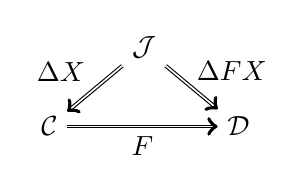
\begin{tikzpicture}[x=0.6cm, y=0.5cm]
    \node (C) at (-2, 0) {$\mathcal{C}$};
    \node (J) at (0, 2) {$\mathcal{J}$};
    \node (D) at (2, 0) {$\mathcal{D}$};
    \draw[->,double] (J)   -- node[ left, yshift=6pt] {$\Delta X$} (C);
    \draw[->,double] (J)   -- node[right, yshift=6pt, xshift=-5pt] {$\ \Delta FX$} (D);
    \draw[->,double] (C)   -- node[below] {$F$} (D);
\end{tikzpicture}
\end{center}
Therefore, $F$ maps a cone $\alpha:\Delta X\Rightarrow G$ to the cone $F\alpha:\Delta FX\Rightarrow FG$.

\begin{definition}
    Let $F:\mathcal{C}\to\mathcal{D}$ and $H:\mathcal{J}\to\mathcal{C}$ be functors.
    \begin{enumerate}
        \item $F$ \textbf{preserves} the limit of $H$ if for all $X\in\ob\mathcal{C}$,
        \[
            \hom_{[\mathcal{J}, \mathcal{C}]}(\Delta-, H)\cong\hom_\mathcal{C}(-, X)
        \]
        implies
        \[
            \hom_{[\mathcal{J}, \mathcal{D}]}(\Delta-, FH) \cong \hom_\mathcal{D}(-, FX).
        \]
        \item $F$ \textbf{reflects} the limit of $H$ if for all $X\in\ob\mathcal{C}$,
        \[
            \hom_{[\mathcal{J}, \mathcal{D}]}(\Delta-, FH) \cong \hom_\mathcal{D}(-, FX)
        \]
        implies
        \[
            \hom_{[\mathcal{J}, \mathcal{C}]}(\Delta-, H)\cong\hom_\mathcal{C}(-, X).
        \]
        \item $F$ is said to be \textbf{continuous} if it preserves all limits, and \textbf{cocontinuous} if it preserves all colimits.
    \end{enumerate}
\end{definition}

Note that a continuous functor preserves not only limit objects, but also the limit cone.

\begin{property}
\label{hom are conti.}
    hom functors are continuous.
    Moreover,
    \[
        \lim\hom_\mathcal{C}(-, F(-)) \cong \hom_\mathcal{C}(-, \lim F).
    \]
\end{property}
\begin{proof}
    If $\hom_{[\mathcal{J}, \mathcal{C}]}(\Delta-, F)\cong\hom_\mathcal{C}(-, \lim F)$, then
    \[
        \lim\hom_\mathcal{C}(-, F(-)) \cong \hom_{[\mathcal{J}, \mathcal{C}]}(\Delta-, F) \cong \hom_\mathcal{C}(-, \lim F)
    \]
    and hence
    \begin{align*}
        \hom_{[\mathcal{J}, \textbf{Set}]}(\Delta-, \hom_\mathcal{C}(X, F-)) 
        & \cong  \hom_{\textbf{Set}}(-, \lim\hom_\mathcal{C}(X, F-)) \\ 
        % & \cong  \hom_{\textbf{Set}}(-, \hom_{[\mathcal{J}, \textbf{Set}]}(\Delta 1, \hom_\mathcal{C}(X, F-))) \\ 
        % & \cong  \hom_{\textbf{Set}}(-, \hom_{[\mathcal{J}, \mathcal{C}]}(\Delta X, F)) \\ 
        & \cong  \hom_{\textbf{Set}}(-, \hom_\mathcal{C}(X, \lim F)).
    \end{align*}
    Dually, $\lim\hom_\mathcal{C}(F^{op}(-), -) \cong \hom_\mathcal{C}(\lim F^{op}, -)$ if $\lim F^{op}$ exists.
\end{proof}

\begin{theorem}
    Let $F\dashv G$ be an adjunction.
    \begin{enumerate}
        \item (RAPL) The right adjoint functor $G$ is continuous.
        \item (LAPC) The left adjoint functor $F$ is cocontinuous.
    \end{enumerate}
\end{theorem}
\begin{proof}
    (1).
    If the limit of $H:\mathcal{J}\to\mathcal{D}$ exists, then
    \begin{align*}
        \hom_\mathcal{C}(-, G\lim H) 
        & \cong \hom_\mathcal{D}(F-, \lim H) & F\dashv G, \\
        & \cong \lim\hom_\mathcal{D}(F-, H(-)) & \text{by } \ref{hom are conti.}, \\
        & \cong \lim\hom_\mathcal{C}(-, GH(-)) & F\dashv G, \\
        & \cong \hom_{[\mathcal{J}, \mathcal{D}]}(\Delta -, GH) & \text{by } \ref{limit}.
    \end{align*}
\end{proof}

Therefore, internal homs are continuous in both variable.

If $\lim$ is itself a functor, then it is continuous.

\begin{property}
    Any fully faithful functor reflects all limits and colimits.
\end{property}
\begin{proof}
    Let $F:\mathcal{C}\to\mathcal{D}$ be fully faithful, then $\hom_\mathcal{C}(-, -)\cong\hom_\mathcal{D}(F-, F-)$.
    If $FX\cong\lim FH$, then
    \begin{align*}
        \hom_\mathcal{C}(-, X) 
        & \cong \hom_\mathcal{D}(F-, FX) 
          \cong \hom_{[\mathcal{J}, \mathcal{D}]}(\Delta F-, FH) \\
        & \cong \lim\hom_\mathcal{D}(F-, FH(-)) 
          \cong \lim\hom_\mathcal{C}(-, H(-)) \\
        & \cong \hom_{[\mathcal{J}, \mathcal{C}]}(\Delta-, H).
    \end{align*}
\end{proof}

\begin{definition}
    A functor $F:\mathcal{C}\to\mathcal{D}$ \textbf{creates} a limit if it preserves and reflects the limit.
\end{definition}

\begin{property}
    Yoneda embeddings create all limit.
\end{property}
\begin{proof}
    Since Yoneda embeddings are fully faithful, they reflect all limit.
    By Proposition \ref{limit} and Proposition \ref{hom are conti.}, they preserve all limit.
\end{proof}

\begin{property}
    Any equivalence creates all limits and colimits.
\end{property}

\subsection{Products and Equalizers}

Note that every discrete category can be considered as a set.

\begin{definition}
    Let $\mathcal{J}$ be a discrete category and $F:\mathcal{J}\to\mathcal{C}$ be a functor.
    \begin{enumerate}
        \item The limit of $F$ is called the \textbf{product}, denoted as $\prod_\mathcal{J}F$.
        \item[] The components of the limit cone $\pi$ are called the \textbf{projections}.
        \item The colimit of $F^{op}$ is called the \textbf{coproduct}, denoted as $\coprod_\mathcal{J}F$.
        \item[] The components of the colimit cone $\iota$ are called the \textbf{injections}.
        % \item A \textbf{product category} is a category that admits all product.
        % \item If $\prod_\mathcal{J}F\cong\coprod_\mathcal{J}F$, it is called the \textbf{direct sum},  denoted as $\bigoplus_\mathcal{J}F$.
    \end{enumerate}
\end{definition}

If $\mathcal{J}$ is discrete, an object/morphism in $[\mathcal{J}, \mathcal{C}]$ is just a $\ob\mathcal{J}$-indexed family of object/morphisms.

\begin{property}
    The following are equivalent:
    \begin{enumerate}
        \item $\mathcal{C}$ is a finite product category.
        \item $\mathcal{C}$ admits the empty product and all binary product.
    \end{enumerate}
\end{property}
\begin{proof}
    The product of one object is the identity. 
    Suppose that $\times:\mathcal{C}^2\to\mathcal{C}$ is the binary product and $\pi_i:\prod_{n-1} F\to F_i$ are the projections for $\{F_i\}_{i=0}^{n-1}$.
    Then $F_n\times\prod_{n-1}F$ is the product of $\{F_i\}_{i=0}^n$, where the limit cone is
    \begin{center}
    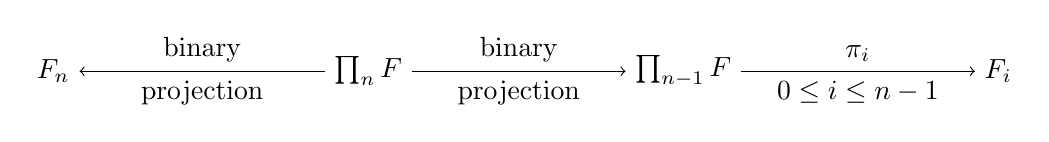
\begin{tikzpicture}[x=1cm, y=0.5cm]
        \node (nF)  at ( 0, 0) {$\prod_nF$};
        \node (n1F) at ( 4, 0) {$\prod_{n-1}F$};
        \node (Fn)  at (-4, 0) {$F_n$};
        \node (Fi)  at ( 8, 0) {$F_i$};
        \draw[->] (n1F) -- node[above]{$\pi_i$} node[below]{$0\le i\le n-1$} (Fi);
        \draw[->] (nF) -- node[above]{binary} node[below]{projection} (n1F);
        \draw[->] (nF) -- node[above]{binary} node[below]{projection} (Fn);
    \end{tikzpicture}
    \end{center}
\end{proof}

Dually, $\mathcal{C}$ admits all finite coproduct if and only if $\mathcal{C}$ admits the empty coproduct and all binary coproduct.

\begin{definition}
    Let $\mathcal{J}$ be a category with the structure
    \begin{center}
    \begin{tikzpicture}[x=1cm, y=0.3cm]
        \node (0) at (0, 0) {$*$};
        \node (1) at (2, 0) {$*$};
        \node (2) at (4, 0) {$*$};
        \draw[->] (0) edge node[above]{1} (1);
        \draw[->] (2) edge node[above]{2} (1);
    \end{tikzpicture}
    \end{center}
    \begin{enumerate}
        \item The limit of the functor $X\xrightarrow{F_1}Z\xleftarrow{F_2}Y$ is called the \textbf{pullback}.
        \item The colimit of the functor $X\xleftarrow{F_1}Z\xrightarrow{F_2}Y$ is called the \textbf{pushout}.
    \end{enumerate}
\end{definition}

A cone $\phi:\Delta A\to F$ for the functor $X\xrightarrow{F_1}Z\xleftarrow{F_2}Y$ is a pair of morphisms $X\xleftarrow{\phi_1}A\xrightarrow{\phi_2}Y$ such that the following commute:
\begin{center}
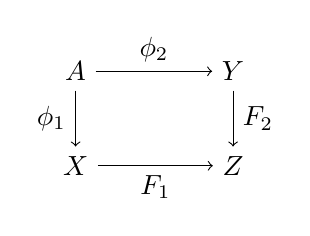
\begin{tikzpicture}[x=1cm, y=0.6cm]
    \node (X) at (0, 0) {$X$};
    \node (Z) at (2, 0) {$Z$};
    \node (Y) at (2, 2) {$Y$};
    \node (lim) at (0, 2) {$A$};
    \draw[->] (X) -- node[below] {$F_1$} (Z);
    \draw[->] (Y) -- node[right] {$F_2$} (Z);
    \draw[->] (lim) -- node[ left] {$\phi_1$} (X);
    \draw[->] (lim) -- node[above] {$\phi_2$} (Y);
\end{tikzpicture}
\end{center}

\begin{definition}
    Let $\mathcal{J}$ be a \textbf{parallel pair}: a category with the structure
    \begin{center}
    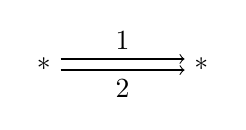
\begin{tikzpicture}[x=1cm, y=0.3cm]
        \node (0) at (0, 0) {$*$};
        \node (1) at (2, 0) {$*$};
        \draw[->, transform canvas={yshift=2pt}] (0) -- node[above]{1} (1);
        \draw[->, transform canvas={yshift=-2pt}] (0) -- node[below]{2} (1);
    \end{tikzpicture}
    \end{center}
    Let $F:\mathcal{J}\to\mathcal{C}$ be a functor, with $F_1, F_2:X\to Y$.
    \begin{enumerate}
        \item The limit of $F$ is called the \textbf{equalizer}, denoted as $\text{eq}(F_1, F_2)$.
        \item The colimit of $F^{op}$ is called the \textbf{coequalizer}, denoted as $\text{coeq}(F_1, F_2)$.
    \end{enumerate}
\end{definition}

A cone $\phi:\Delta A\Rightarrow F$ for the functor $F_1, F_2:X\to Y$ is a morphism $\phi:A\to X$ such that $F_1\circ\phi=F_2\circ\phi$.
For the limit cone $\epsilon:\text{eq}(F_1, F_2)\to X$, the diagram:
\begin{center}
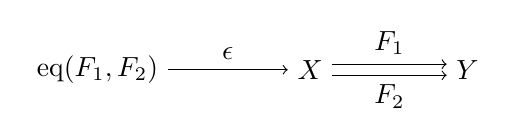
\begin{tikzpicture}[x=1cm, y=0.3cm]
    \node (0) at (0, 0) {$X$};
    \node (1) at (2, 0) {$Y$};
    \node (-1) at (-2.7, 0) {$\text{eq}(F_1, F_2)$};
    \draw[->, transform canvas={yshift=2pt}] (0) -- node[above]{$F_1$} (1);
    \draw[->, transform canvas={yshift=-2pt}] (0) -- node[below]{$F_2$} (1);
    \draw[->] (-1) -- node[above]{$\epsilon$} (0);
\end{tikzpicture}
\end{center}

is called a \textbf{equalizer diagram}.

\begin{corollary}
    All equalizers are monic, all coequalizers are epic.
\end{corollary}

In fact, any limit can be characterized using products and equalizers.

Define the functors 
\begin{center}
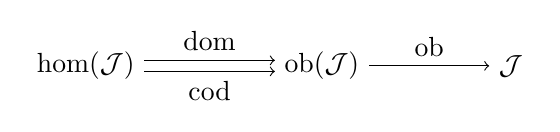
\begin{tikzpicture}[x=1.2cm, y=0.3cm]
    \node (0) at (-2.5, 0) {$\hom(\mathcal{J})$};
    \node (1) at (2, 0) {$\mathcal{J}$};
    \node (-1) at (0, 0) {$\ob(\mathcal{J})$};
    \draw[->, transform canvas={yshift=2pt}] (0) -- node[above]{dom} (-1);
    \draw[->, transform canvas={yshift=-2pt}] (0) -- node[below]{cod} (-1);
    \draw[->] (-1) -- node[above]{$\ob$} (1);
\end{tikzpicture}
\end{center}
where $\ob$ maps each object to itself, dom maps a morphism $f:X\to Y$ to its domain $X$, and cod maps $f:X\to Y$ to its codomain $Y$.

\begin{theorem}
    Let $F:\mathcal{J}\to\mathcal{C}$ be a functor.
    Suppose that 
    \begin{enumerate}
        \item $\text{F}=F\circ\ob$ and $\mathcal{F}:\text{F\,dom}\Rightarrow\text{F\,cod}:f\mapsto Ff$.
        \item $\prod\text{F}$ and $\prod \text{F\,cod}$ exists, and $\pi:\Delta\prod \text{F}\Rightarrow\text{F}$ is the projection.
        \item $\mathcal{I}$ is the category $*\rightrightarrows*$, and $f:\mathcal{I}\to\mathcal{C}$ is the functor defined by
        \begin{center}
        \begin{tabular}{ccc}
            $\hom_{[\hom(\mathcal{J}), \mathcal{C}]}(\Delta\prod\text{F}, \text{F\,cod})$ & $\cong$ & $\hom_\mathcal{C}(\prod\text{F}, \prod \text{F\,cod})$ \\[2pt]
            $\pi\,\text{cod}$ & $\leftrightarrows$ & $f_1$ \\[2pt]
            $\mathcal{F}\circ\pi\,\text{dom}$ & $\leftrightarrows$ & $f_2$
        \end{tabular} 
        \end{center}
    \end{enumerate}
    Then $\hom_{[\mathcal{J}, \mathcal{C}]}(\Delta-, F)\cong\hom_{[\mathcal{I}, \mathcal{C}]}(\Delta-, f)$.
\end{theorem}
\begin{proof}
    Consider the correspondence:
        \begin{center}
        \begin{tabular}{ccc}
            $\hom_{[\ob\mathcal{J}, \mathcal{C}]}(\Delta X, \text{F})$ & $\cong$ & $\hom_\mathcal{C}(X, \prod\text{F})$ \\[2pt]
            $\phi^\sharp=\pi\circ\Delta\phi^\flat$ & $\leftrightarrows$ & $\phi^\flat$
        \end{tabular} 
        \end{center}
    Then
    \begin{align*}
        \phi^\flat\in\hom_{[\mathcal{I}, \mathcal{C}]}(\Delta X, f)
        & \iff f_1\circ\phi^\flat = f_2\circ\phi^\flat \\
        & \iff \pi\,\text{cod}\circ\Delta\phi^\flat = \mathcal{F}\circ\pi\,\text{dom}\circ\Delta\phi^\flat \\
        & \iff \phi^\sharp=\pi\circ\Delta\phi^\flat\in\hom_{[\mathcal{J}, \mathcal{C}]}(\Delta X, F),
    \end{align*}
    and the naturality follows from $\hom_{[\ob\mathcal{J}, \mathcal{C}]}(\Delta -,\text{F})\cong\hom_\mathcal{C}(-, \prod\text{F})$.
\end{proof}

\begin{corollary}
    The following are equivalent:
    \begin{enumerate}
        \item $\mathcal{C}$ is complete.
        \item $\mathcal{C}$ admits all products and all equalizers.
    \end{enumerate}
\end{corollary}

Dually, $\mathcal{C}$ is cocomplete if and only if $\mathcal{C}$ has all coproducts and coequalizers.

\subsection{Adjoint Functor Theorems}

We do not distinguish between the morphism $(1_X, \phi)$ and $\phi$ in $\Delta X\downarrow G$.

\begin{lemma}
\label{comma limit}
    Let $G:\mathcal{D}\to\mathcal{C}$ be continuous and $X\in\ob\mathcal{C}$.
    The functor
    \[
        U:\Delta X\downarrow G\to\mathcal{D}:(f:X\to GA)\mapsto A:\phi\mapsto\phi.
    \]
    creates all limits.
    In particular, $\Delta X\downarrow G$ is complete if $\mathcal{D}$ is.
\end{lemma}
\begin{proof}
    Let $F:\mathcal{J}\to\Delta X\downarrow G$ be a functor.
    Then every component of a cone $\phi^\sharp:\Delta f\Rightarrow F$ has the form $\phi^\sharp_i:Uf\to UFi$.
    Given $l=\lim F$ and
    \begin{center}
    \begin{tabular}{ccc}
        $\hom_{[\mathcal{J}, \Delta X\downarrow G]}(\Delta f, F)$ & $\cong$ & $\hom_{\Delta X\downarrow G}(f, l)$ \\[2pt]
        $\phi^\sharp$ & $\leftrightarrows$ & $\phi^\flat$
    \end{tabular} 
    \end{center}
    Given the correspondence
    \begin{center}
    \begin{tabular}{ccc}
        $\hom_{[\mathcal{J}, \mathcal{D}]}(\Delta A, UF)$ & $\cong$ & $\hom_\mathcal{D}(A, Ul)$ \\[2pt]
        $\phi^\sharp$ & $\leftrightarrows$ & $\phi^\flat$
    \end{tabular} 
    \end{center}
    Then 
    \begin{align*}
        \phi^\flat \in \hom_{\Delta X\downarrow G}(f, l) 
        & \iff 
    \end{align*}
\end{proof}

\begin{property}
    If $\mathcal{D}$ is complete and $G:\mathcal{D}\to\mathcal{C}$ is continuous, then $G$ admits left adjoint.
\end{property}
\begin{proof}
    Since the limit of the identity on $\Delta X\downarrow G$ exists and is the initial object, the universal property holds for all $X\in\ob\mathcal{C}$.
\end{proof}

\begin{definition}
    Let $\mathcal{D}$ be a category.
    \begin{enumerate}
        \item A set $S$ of objects is \textbf{jointly weakly initial} if for every object $Y$, there exists $X\in S$ such that $\hom_\mathcal{D}(X,Y)\ne\varnothing$.
        \item A \textbf{joint equalizer} is a limit of a set of parallel morphisms.
    \end{enumerate}
\end{definition}

A set of parallel morphisms is a category with the structure
\begin{center}
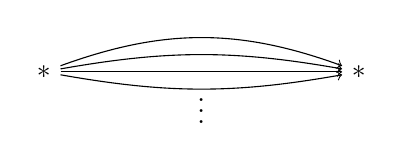
\begin{tikzpicture}[x=2cm, y=0.1cm]
    \node (0) at (0, 0) {$*$};
    \node (1) at (2, 0) {$*$};
    \draw[->, bend right= 10] (0) edge (1);
    \draw[->, bend right=  0] (0) edge node[below]{$\vdots$} (1);
    \draw[->, bend right=-10] (0) edge (1);
    % \draw[->, bend right= -7] (0) edge (1);
    \draw[->, bend right=-20] (0) edge (1);
\end{tikzpicture}
\end{center}
A joint equalizer is then a limit of a functor defined on it.

\begin{theorem}[Freyd]
    Let $\mathcal{D}$ be a category that admits all joint equalizer, $G:\mathcal{D}\to\mathcal{C}$ be a continuous functor.
    Then the following are equivalent:
    \begin{enumerate}
        \item $G$ has a left adjoint.
        \item For each $X\in\ob\mathcal{C}$, there is a jointly weakly initial set $S_X$ in $\Delta X\downarrow G$ such that $\mathcal{D}$ admit the product on $S_X$.
    \end{enumerate}
\end{theorem}

\section{Monoidal Category}

\subsection{2-multicategory}

\begin{definition}
    A \textbf{2-multicategory} $\mathcal{M}$ consists of:
    \begin{enumerate}
        \item A set $\ob\mathcal{M}$ of objects.
        \item[] A tuple $\textbf{X}$ of objects $X_1, \cdots, X_k\in\ob\mathcal{M}$ is called a \textbf{vector}.
        \item For vector $\textbf{X}$ and object $Y$, a \textbf{hom-category} $\mathcal{M}(\textbf{X}; Y)$.
        \item For vectors $\textbf{X}_1, \cdots, \textbf{X}_k$, $k$-tuple $\textbf{Y}=(Y_1, \cdots, Y_k)$ and object $Z$, a functor
        \[
            \circ: \mathcal{M}(\textbf{Y}; Z)\times\prod\mathcal{M}(\textbf{X}_i; Y_i)\to\mathcal{M}(\textbf{X}_1, \cdots, \textbf{X}_k; Z)
        \]
        called \textbf{composition}, such that
        \[
            f\circ(g_1\circ\textbf{h}_1, \cdots, g_k\circ\textbf{h}_k)
            = (f\circ\textbf{g})\circ(\textbf{h}_1, \cdots, \textbf{h}_k).
        \]
        \item For object $X$, an \textbf{identity} $1_X\in\mathcal{M}(X; X)$ such that
        \[
            1_X\circ\textbf{g} = \textbf{g} 
            \quad\text{and}\quad
            f\circ(1_{X_1}, \cdots, 1_{X_k}) = f.
        \]
    \end{enumerate}
\end{definition}

\begin{definition}
    Let $\mathcal{M}$ be a 2-multicategory.
    \begin{enumerate}
        \item $\mathcal{M}$ is called a \textbf{2-operad} if $\mathcal{M}$ is a singleton.
        \item $\mathcal{M}$ is \textbf{lax coherence} if all its hom-categories are connected and thin.
        \item $\mathcal{M}$ is \textbf{coherence} if all its hom-categories are connected and thin groupoid.
    \end{enumerate}
\end{definition}

\begin{definition}
    A \textbf{2-multifunctor} $F:\mathcal{M}\to\mathcal{N}$ consist of:
    \begin{enumerate}
        \item A function $F:\ob\mathcal{M}\to\ob\mathcal{N}$.
        \item For vector $\textbf{X}$ and object $Y$ in $\mathcal{M}$, a functor
        \[
            F_{\textbf{X}, Y}:\mathcal{M}(\textbf{X}; Y)\to\mathcal{N}(FX_1, \cdots, FX_k; FY).
        \]
        \item Composition and identities are preserved.
    \end{enumerate}
\end{definition}

% \subsection{Coherence}


% \begin{definition}
%     Let $n_1, \cdots, n_k\in\mathbb{N}$.
%     \begin{enumerate}
%         \item Let $T_i:\mathcal{C}^{n_i}\to\mathcal{D}$ for each $i$, define
%         \[
%             \textbf{T}:\mathcal{C}^{\sum n}\to\mathcal{D}^k:(\textbf{x}_1, \cdots, \textbf{x}_k)\mapsto(T_1\textbf{x}_1, \cdots, T_k\textbf{x}_k).
%         \]
%         \item Let $\alpha_i:T_i\Rightarrow U_i:\mathcal{C}^{n_i}\to\mathcal{D}$ for each $i$, define
%         \[
%             \pmb{\alpha}:\textbf{T}\Rightarrow\textbf{U}:(\textbf{x}_1, \cdots, \textbf{x}_k)\mapsto(\alpha_1\textbf{x}_1, \cdots, \alpha_k\textbf{x}_k).
%         \]
%     \end{enumerate}
% \end{definition}

% \begin{definition}
%     Let $\iota:\mathcal{D}\to\mathcal{C}$ be a category.
%     \begin{enumerate}
%         \item A \textbf{signature} is a functor $\Sigma:\mathbb{N}\to\textbf{CAT}$.
%         \item A \textbf{interpretation} is a natural transformation $\sigma:\Sigma\Rightarrow[\mathcal{C}^-, \mathcal{C}]$.
%         \item A subcategory $\mathcal{D}$ of $\mathcal{C}$ is said to be \textbf{closed} under $F:\mathcal{C}^k\to\mathcal{C}$ if it defines an operator on $\mathcal{D}$.
%         \item A 
%     \end{enumerate}
% \end{definition}

% \begin{definition}
%     Let $\mathcal{C}$ be a category.
%     \begin{enumerate}
%         \item Define $\op\mathcal{C}=\coprod_{i\in\mathbb{N}}[\mathcal{C}^i, \mathcal{C}]$ be the \textbf{category of operators}.
%         \item Let $F:\mathcal{C}^k\to\mathcal{C}$ be an operator.
%         Define
%         \[
%             \op F:(\op\mathcal{C})^k\to\op\mathcal{C}:
%             (T_1, \cdots, T_k)\mapsto F\textbf{T}:
%             (\alpha_1, \cdots, \alpha_k)\mapsto F\pmb{\alpha}.
%         \]
%         \item Let $\alpha:F\Rightarrow G:\mathcal{C}^k\to\mathcal{C}$.
%         Define
%         \[
%             \op\alpha:\op F\Rightarrow\op G:(T_1, \cdots, T_k)\mapsto\alpha\textbf{T}.
%         \]
%     \end{enumerate}
% \end{definition}

% For example, set $\Sigma_0=\{T:\mathcal{C}^2\to\mathcal{C}, S:\mathcal{C}\to\mathcal{C}\}$ and 
% \[
%     \Sigma_1=\{\alpha:T\Rightarrow T(S, 1_\mathcal{C}), \beta:T(1_\mathcal{C}, S)\Rightarrow T\}.
% \]
% Then $S(\alpha):S(T)\Rightarrow ST(S, 1_\mathcal{C})$ is a morphism in $F(\Sigma)$.

% If $\Sigma=(T, S; \alpha, \beta)$ is coherence, then the diagram
% \begin{center}
% \begin{tikzpicture}[x=2cm, y=0.7cm]
%     \node (T1S) at (0, 2) {$T(1_\mathcal{C}, S)$};
%     \node (T)   at (2, 2) {$T$};
%     \node (TSS) at (0, 0) {$T(S, S)$};
%     \node (TS1) at (2, 0) {$T(S, 1_\mathcal{C})$};
%     \draw[->] (T1S)  -- node[above] {$\beta$} (T);
%     \draw[->] (T)    -- node[right] {$\alpha$} (TS1);
%     \draw[->] (T1S)  -- node[ left] {$\beta(S, 1_\mathcal{C})$} (TSS);
%     \draw[->] (TSS)  -- node[below] {$\alpha(1_\mathcal{C}, S)$} (TS1);
% \end{tikzpicture}
% \end{center}
% is commute in $F(\Sigma)$.

% \begin{definition}
%     Let $\mathcal{C}'$ and $\mathcal{D}'$ be closed subcategories of $\text{Fct}(\mathcal{C})$ and $\text{Fct}(\mathcal{D})$, respectively.
%     A functor $F:\mathcal{C}\to\mathcal{D}$ is called \textbf{coherence} if
% \end{definition}

% \begin{definition}
%     For each $n\in\mathbb{N}$, define the \textbf{permutation functor}
%     \[
%         S_n\to\textbf{Cat}:*\mapsto[\mathcal{C}^n, \mathcal{C}]:\sigma\mapsto\sigma-
%     \]
%     where $\sigma-:[\mathcal{C}^n, \mathcal{C}]\to[\mathcal{C}^n, \mathcal{C}]$ is defined by
%     \begin{enumerate}
%         \item $\sigma F:\mathcal{C}^n\to\mathcal{C}:(x_1, \cdots, x_n)\mapsto F(x_{\sigma(1)}, \cdots, x_{\sigma(n)})$.
%         \item $\sigma \alpha:\sigma F\Rightarrow\sigma G:(x_1, \cdots, x_n)\mapsto \alpha(x_{\sigma(1)}, \cdots, x_{\sigma(n)})$.
%     \end{enumerate}
% \end{definition}

% \begin{definition}
%     Let $\mathcal{C}$ be a category.
%     \begin{enumerate}
%         \item A closed subcategory $\mathcal{C}'=\coprod_{n\in\mathbb{N}}\mathcal{C}'_n$ of $\text{Fct}(\mathcal{C})$ is said to be \textbf{permuted closed} if for all $n\in\mathbb{N}$, the permutation functor induced a functor
%         \[
%             S_n\to\textbf{Cat}:*\mapsto\mathcal{C}'_n.
%         \]
%         \item The \textbf{free permuted $\Sigma$-category} $F_p(\Sigma)$ is the smallest permuted closed subcategory of $\text{Fct}(\mathcal{C})$ containing the signature $\Sigma$.
%         \item $\Sigma$ is said to be \textbf{permuted coherence} if every diagram in $F_p(\Sigma)$ is commute.
%     \end{enumerate}
% \end{definition}

% \subsection{Monoidal Category}

% Write $-$ for the identity functor $1_\mathcal{C}:\mathcal{C}\to\mathcal{C}$.

% \begin{definition}
%     Let $\otimes:\mathcal{C}^2\to\mathcal{C}$ and $I:\mathcal{C}^0\to\mathcal{C}$ be functors.
%     \begin{enumerate}
%         \item An isomorphism $a:(-\otimes-)\otimes-\cong-\otimes(-\otimes-)$ is called \textbf{associator}.
%         \item An isomorphism $l:I\otimes-\cong-$ is called \textbf{left unitor}.
%         \item An isomorphism $r:-\otimes I\cong-$ is called \textbf{right unitor}.
%         \item An isomorphism $b:\otimes\cong(12)\otimes$ is called \textbf{braiding}, where $(12)\in S_2$.
%     \end{enumerate}
% \end{definition}

% \begin{definition}
%     Define $\otimes, I, a, l, r, b$ as above.
%     \begin{enumerate}
%         \item A category is called \textbf{monoidal} if
%         \[
%             (\otimes, I; a, l, r)
%         \]
%         is coherence, denoted $(\mathcal{V}, \otimes, I, a, l, r)$ or $(\mathcal{V}, \otimes, I)$.
%         \item A category is called \textbf{symmetric monoidal} if
%         \[
%             (\otimes, I;a, l, r, b)
%         \]
%         is permuted coherence.
%     \end{enumerate}
% \end{definition}

\subsection{Cartesian and Tensor}

\begin{property}
    If $\mathcal{C}$ admits all finite products, then $(\mathcal{C}, \times, 1)$ is a monoidal category.
\end{property}
\begin{proof}
    Since the left diagram commutes, the right diagram commutes:
    \begin{center}
    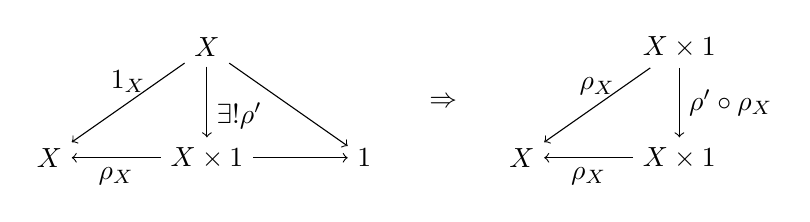
\begin{tikzpicture}[x=1cm, y=0.7cm]
        \node (X1) at (0, 0) {$X\times 1$};
        \node (X)  at (-2, 0) {$X$};
        \node (1)  at ( 2, 0) {$1$};
        \node (uX)  at ( 0, 2) {$X$};
        \draw[->] (X1)  -- node[below]{$\rho_X$} (X);
        \draw[->] (X1)  -- (1);
        \draw[->] (uX)  -- node[right, pos=0.7]{$\exists!\rho'$} (X1);
        \draw[->] (uX)  -- node[above]{$1_X$} (X);
        \draw[->] (uX)  -- (1);
        \node (arrow) at (3, 1) {$\Rightarrow$};
        \node (X1') at (6, 0) {$X\times 1$};
        \node (X')  at (4, 0) {$X$};
        \node (uX1)  at ( 6, 2) {$X\times 1$};
        \draw[->] (X1')  -- node[below]{$\rho_X$} (X');
        \draw[->] (uX1)  -- node[right]{$\rho'\circ\rho_X$} (X1');
        \draw[->] (uX1)  -- node[above]{$\rho_X$} (X');
    \end{tikzpicture} 
    \end{center}
    The uniqueness assert that $\rho'\circ\rho_X=1_X$ and $\rho:-\times 1\cong -$.
\end{proof}

\begin{definition}
    A monoidal category $(\mathcal{V}, \otimes, I)$ is said to be \textbf{closed} if $\otimes$ is given by the tensor-hom adjunction.
\end{definition}

\begin{property}
    Let $(\mathcal{V}, \otimes, I)$ be a closed monoidal category and $[-, -]$ be the internal hom, then
    \[
        [-\otimes-, -] \cong [-, [-, -]].
    \]
\end{property}
\begin{proof}
    Since
    \begin{align*}
        \hom_\mathcal{V}(-, [-\otimes-, -])
        & \cong \hom_\mathcal{V}(-\otimes(-\otimes-), -) \\
        & \cong \hom_\mathcal{V}((-\otimes-)\otimes-, -) \\
        & \cong \hom_\mathcal{V}(-\otimes-, [-, -]) \\
        & \cong \hom_\mathcal{V}(-, [-, [-, -]]),
    \end{align*}
    by corollary \ref{227}, $[-\otimes-, -] \cong [-, [-, -]]$.
\end{proof}

\subsection{Terminology and Constructions}

\begin{corollary}
    Let $\mathcal{C}$ be a category.
    \begin{enumerate}
        \item $([\mathcal{C}, \mathcal{C}], *, 1_\mathcal{C})$ is monoidal, where $*$ is the horizontal composition.
        \item If $(\mathcal{V}, \otimes, I)$ is monoidal, then so is $([\mathcal{C}, \mathcal{V}], \otimes', \Delta I)$ with
        \[
            (F\otimes' G)(-) = (F-)\otimes(G-).
        \]
    \end{enumerate}
\end{corollary}

\subsection{Appendix: Coherence Theorem}

\begin{theorem}
    Define $\otimes, I, a, l, r, b$ as before.
    \begin{enumerate}
        \item $(\otimes; a)$ is coherence if and only if the \textbf{pentagon diagram} commute:
        \begin{center}
        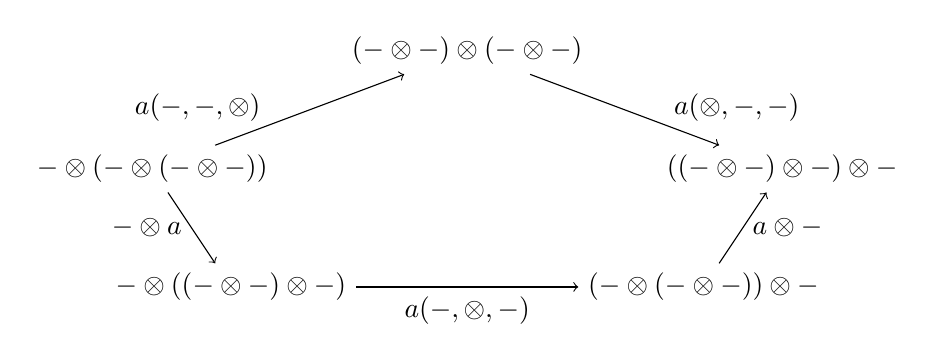
\begin{tikzpicture}[x=1cm, y=1.5cm]
            \node (10) at (1, 0) {$-\otimes((-\otimes-)\otimes-)$};
            \node (01) at (0, 1) {$-\otimes(-\otimes(-\otimes-))$};
            \node (42) at (4, 2) {$(-\otimes-)\otimes(-\otimes-)$};
            \node (81) at (8, 1) {$((-\otimes-)\otimes-)\otimes-$};
            \node (70) at (7, 0) {$(-\otimes(-\otimes-))\otimes-$};
            \draw[->] (01)  -- node[ left]{$-\otimes a$} (10);
            \draw[->] (70)  -- node[right]{$a\otimes-$} (81);
            \draw[->] (01)  -- node[pos=0.2,above]{$a(-, -, \otimes)\hspace{4em}$} (42);
            \draw[->] (42)  -- node[pos=0.8,above]{$\hspace{4em}a(\otimes, -, -)$} (81);
            \draw[->] (10)  -- node[below]{$a(-, \otimes, -)$} (70);
        \end{tikzpicture} 
        \end{center}
        \item $(\otimes, I; a, l, r)$ is coherence if and only if $(\otimes; a)$ is coherence and the \textbf{triangle diagram} commute:
        \begin{center}
        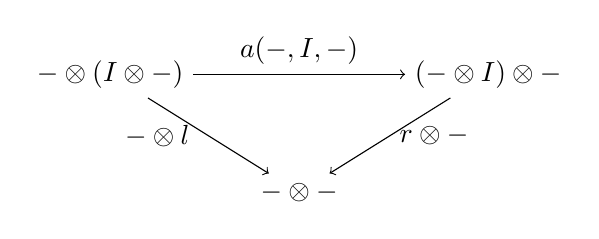
\begin{tikzpicture}[x=1.2cm, y=1.5cm]
            \node (01) at (0, 1) {$-\otimes(I\otimes-)$};
            \node (20) at (2, 0) {$-\otimes-$};
            \node (41) at (4, 1) {$(-\otimes I)\otimes-$};
            \draw[->] (01)  -- node[ left]{$-\otimes l\ $} (20);
            \draw[->] (41)  -- node[right]{$r\otimes-$} (20);
            \draw[->] (01)  -- node[above]{$a(-, I, -)$} (41);
        \end{tikzpicture} 
        \end{center}
        \item $(\otimes; a, b)$ is permuted coherence if and only if $(\otimes; a)$ is coherence and the \textbf{hexagon diagram} commute:
        \begin{center}
        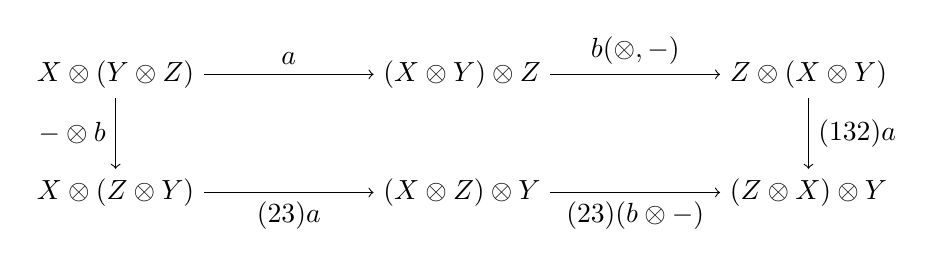
\begin{tikzpicture}[x=2.2cm, y=1.5cm]
            \node (00) at (0, 0) {$X\otimes(Z\otimes Y)$};
            \node (01) at (0, 1) {$X\otimes(Y\otimes Z)$};
            \node (20) at (2, 0) {$(X\otimes Z)\otimes Y$};
            \node (21) at (2, 1) {$(X\otimes Y)\otimes Z$};
            \node (40) at (4, 0) {$(Z\otimes X)\otimes Y$};
            \node (41) at (4, 1) {$Z\otimes(X\otimes Y)$};
            \draw[->] (01)  -- node[ left]{$-\otimes b$} (00);
            \draw[->] (00)  -- node[below]{$(23)a$} (20);
            \draw[->] (20)  -- node[below]{$(23)(b\otimes-)$} (40);
            \draw[->] (41)  -- node[right]{$(132)a$} (40);
            \draw[->] (01)  -- node[above]{$a$} (21);
            \draw[->] (21)  -- node[above]{$b(\otimes, -)$} (41);
        \end{tikzpicture} 
        \end{center}
    \end{enumerate}
\end{theorem}

\section{Enriched Category}

\subsection{Elementary}

Let $(\mathcal{V}, \otimes, I)$ be a monoidal category.

\begin{definition}
    A \textbf{$\mathcal{V}$-category} $\mathcal{C}$ consists of:
    \begin{enumerate}
        \item A set $\ob\mathcal{C}$ of objects.
        \item For $X, Y\in\ob\mathcal{C}$, an object $\mathcal{C}(X, Y)$ in $\mathcal{V}$.
        \item For $X, Y, Z\in\ob\mathcal{C}$, a morphism
        \[
            \circ_{X, Y, Z}:\mathcal{C}(Y, Z)\otimes\mathcal{C}(X, Y)\to\mathcal{C}(X, Z)
        \]
        in $\mathcal{V}$ called \textbf{composition}.
        \item For $X\in\ob\mathcal{C}$, a morphism $i_X:I\to\mathcal{C}(X, X)$ in $\mathcal{V}$ called \textbf{identity}.
    \end{enumerate}
    such that the associative
    \begin{center}
    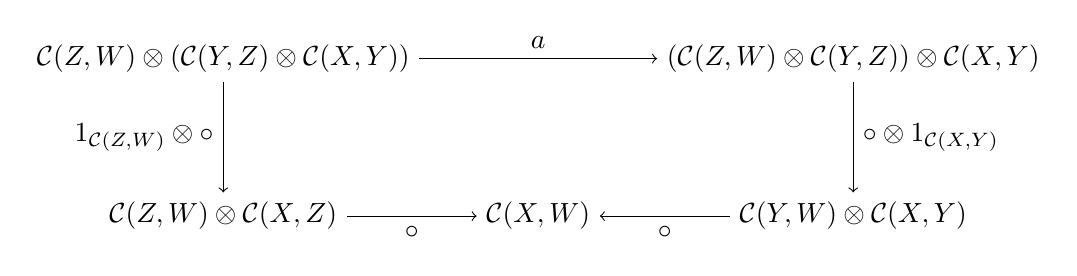
\begin{tikzpicture}[x=2cm, y=1cm]
        \node (40) at (4, 0) {$\mathcal{C}(Y, W)\otimes\mathcal{C}(X, Y)$};
        \node (42) at (4, 2) {$(\mathcal{C}(Z, W)\otimes\mathcal{C}(Y, Z))\otimes\mathcal{C}(X, Y)$};
        \node (20) at (2, 0) {$\mathcal{C}(X, W)$};
        \node (02) at (0, 2) {$\mathcal{C}(Z, W)\otimes(\mathcal{C}(Y, Z)\otimes\mathcal{C}(X, Y))$};
        \node (00) at (0, 0) {$\mathcal{C}(Z, W)\otimes\mathcal{C}(X, Z)$};
        \draw[->] (42)  -- node[right]{$\circ\otimes1_{\mathcal{C}(X, Y)}$} (40);
        \draw[->] (02)  -- node[above]{$a$} (42);
        \draw[->] (00)  -- node[below]{$\circ$} (20);
        \draw[->] (40)  -- node[below]{$\circ$} (20);
        \draw[->] (02)  -- node[ left]{$1_{\mathcal{C}(Z, W)}\otimes\circ$} (00);
    \end{tikzpicture}
    \end{center}
    and the unital hold:
    \begin{center}
    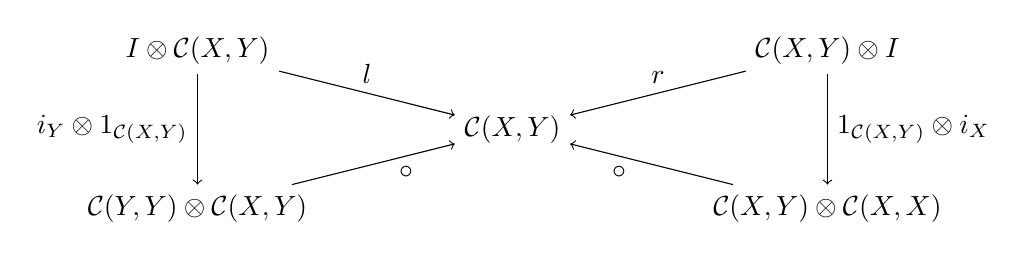
\begin{tikzpicture}[x=2cm, y=1cm]
        \node (40) at (4, 0) {$\mathcal{C}(X, Y)\otimes\mathcal{C}(X, X)$};
        \node (42) at (4, 2) {$\mathcal{C}(X, Y)\otimes I$};
        \node (21) at (2, 1) {$\mathcal{C}(X, Y)$};
        \node (02) at (0, 2) {$I\otimes\mathcal{C}(X, Y)$};
        \node (00) at (0, 0) {$\mathcal{C}(Y, Y)\otimes\mathcal{C}(X, Y)$};
        \draw[->] (42)  -- node[right]{$1_{\mathcal{C}(X, Y)}\otimes i_X$} (40);
        \draw[->] (02)  -- node[above]{$l$} (21);
        \draw[->] (42)  -- node[above]{$r$} (21);
        \draw[->] (00)  -- node[pos=0.7, below]{$\circ$} (21);
        \draw[->] (40)  -- node[pos=0.7, below]{$\circ$} (21);
        \draw[->] (02)  -- node[ left]{$i_Y\otimes1_{\mathcal{C}(X, Y)}$} (00);
    \end{tikzpicture}
    \end{center}
\end{definition}

\begin{definition}
    A \textbf{$\mathcal{V}$-functor} $F:\mathcal{C}\to\mathcal{D}$ consist of:
    \begin{enumerate}
        \item A function $F:\ob\mathcal{C}\to\ob\mathcal{D}$.
        \item For $X, Y\in\ob\mathcal{C}$, a morphism $F_{X, Y}:\mathcal{C}(X, Y)\to\mathcal{D}(FX, FY)$ in $\mathcal{V}$.
    \end{enumerate}
    such that the follwing diagrmas commute:
    \begin{center}
    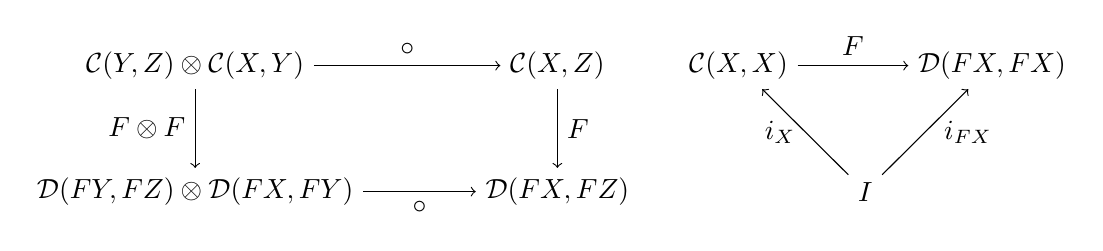
\begin{tikzpicture}[x=2.3cm, y=0.8cm]
        \node (FX) at (0, 2) {$\mathcal{C}(Y, Z)\otimes\mathcal{C}(X, Y)$};
        \node (FY) at (0, 0) {$\mathcal{D}(FY, FZ)\otimes\mathcal{D}(FX, FY)$};
        \node (GX) at (2, 2) {$\mathcal{C}(X, Z)$};
        \node (GY) at (2, 0) {$\mathcal{D}(FX, FZ)$};
        \draw[->] (FX) -- node[above]{$\circ$} (GX);
        \draw[->] (FX) -- node[left] {$F\otimes F$} (FY);
        \draw[->] (FY) -- node[below]{$\circ$} (GY);
        \draw[->] (GX) -- node[right]{$F$} (GY);
        \node (I) at (3.7, 0){$I$};
        \node (C) at (3, 2){$\mathcal{C}(X, X)$};
        \node (D) at (4.4, 2){$\mathcal{D}(FX, FX)$};
        \draw[->] (I) -- node[ left]{$i_X$} (C);
        \draw[->] (I) -- node[right]{\ $i_{FX}$} (D);
        \draw[->] (C) -- node[above]{$F$} (D);
    \end{tikzpicture}
    \end{center}
\end{definition}

\begin{definition}
    A \textbf{$\mathcal{V}$-natural transformation} $\alpha:F\Rightarrow G$ is a function
    \[
        \alpha: \ob(\mathcal{C})\to\hom(\mathcal{V}): X\mapsto(\alpha_X:I\to\mathcal{D}(FX, GX))
    \]
    such that the follwing diagram commute:
    \begin{center}
    \begin{tikzpicture}[x=3cm, y=1.3cm]
        \node (C) at (0, 1) {$\mathcal{C}(X, Y)$};
        \node (CI) at (1, 0) {$\mathcal{C}(X, Y)\otimes I$};
        \node (IC) at (1, 2) {$I\otimes\mathcal{C}(X, Y)$};
        \node (DT) at (2.8, 2) {$\mathcal{D}(FY, GY)\otimes\mathcal{D}(FX, FY)$};
        \node (SD) at (2.8, 0) {$\mathcal{D}(GX, GY)\otimes\mathcal{D}(FX, GX)$};
        \node (D)  at (4, 1) {$\mathcal{D}(FX, GY)$};
        \draw[->] (C) -- node[above, pos=0.3]{$r^{-1}$} (CI);
        \draw[->] (C) -- node[below, pos=0.3]{$l^{-1}$} (IC);
        \draw[->] (CI) -- node[above]{$G\otimes\alpha_X$} (SD);
        \draw[->] (IC) -- node[below]{$\alpha_Y\otimes F$} (DT);
        \draw[->] (DT) -- node[above, pos=0.7]{$\circ$} (D);
        \draw[->] (SD) -- node[below, pos=0.7]{$\circ$} (D);
    \end{tikzpicture}
    \end{center}
\end{definition}

\begin{property}
    If $\mathcal{V}$ is symmetric and closed, then $\mathcal{V}$ is a $\mathcal{V}$-category.
\end{property}

\section{Higher Algebra}

\subsection{Monoid Object}

Let $\mathcal{V}$ be a monoidal category.

\begin{definition}
    A $\mathcal{V}$-category with one object $M$ is called a \textbf{monoid} in $\mathcal{V}$.
\end{definition}

\begin{definition}
    The category of monoids $\Mon\mathcal{V}$ is defined by:
    \begin{enumerate}
        \item $\ob \Mon\mathcal{V}=\{M\in\ob\mathcal{V}\ |\ M\text{ is a monoid in }\mathcal{C}\}$.
        \item $\hom(M, N)=\{F:M\to N\ |\ F\text{ is a $\mathcal{V}$-functor}\}$.
    \end{enumerate}
\end{definition}

\begin{definition}
    Suppose that $M$ is a monoid in a symmetric closed $\mathcal{V}$.
    A $\mathcal{V}$-functor $F:\mathcal{M}\to\mathcal{V}$ is called a \textbf{(left) module} over $M$.
\end{definition}

\subsection{Monad}

Let $\mathcal{C}$ be a category.
Note that $([\mathcal{C}, \mathcal{C}], *, 1_\mathcal{C})$ is monoidal.

\begin{definition}
    A \textbf{monad} in $\mathcal{C}$ is a monoid $T$ in $[\mathcal{C}, \mathcal{C}]$.
    \begin{enumerate}
        \item The identity $\eta:1_\mathcal{C}\Rightarrow T$ is called the \textbf{unit}.
        \item The composition $\mu:T\circ T\Rightarrow T$ is called the \textbf{multiplication}.
    \end{enumerate}
\end{definition}

\begin{lemma}
    Let $F\dashv G$ be an adjunction.
    Then $GF:\mathcal{C}\to\mathcal{C}$ is a monad.
\end{lemma}
\begin{proof}
    Set $\eta:1_\mathcal{C}\Rightarrow GF$ be the unit and $\mu=G\epsilon F$.
\end{proof}

\end{CJK}
\end{document}